
\documentclass{article}
\usepackage[utf8x]{inputenc} 
\usepackage{amsmath,bm}
\usepackage{float}
\usepackage[english]{babel}
\usepackage{natbib}
\usepackage{booktabs}
\usepackage{setspace}\doublespacing
\setlength{\parskip}{0.5em}
\usepackage[left]{lineno}\linenumbers
\usepackage[a4paper, total={6in, 8in}]{geometry}
\usepackage{isomath}
\usepackage{amsmath}
\usepackage{mathtools}
\usepackage{longtable}
\usepackage[font={footnotesize,it}]{caption}
\usepackage{rotating}
\usepackage[colorinlistoftodos]{todonotes}

\usepackage{totcount} \newtotcounter{citnum}
\def\oldbibitem{} \let\oldbibitem=\bibitem
\def\bibitem{\stepcounter{citnum}\oldbibitem}


\begin{document}


\begin{center}
\large
\textbf{Social environments and their eco-evolutionary dynamics: from density regulation to frequency-dependent selection}
\end{center}

\begin{center}
	Yimen G. Araya-Ajoy\textsuperscript{1,2}, Myranda Murray\textsuperscript{1}, Steinar Engen\textsuperscript{1}, Bernt-Erik Sæther\textsuperscript{1}, Jonathan Wright\textsuperscript{1}
\end{center}

\bigskip
\noindent \textsuperscript{\textbf{1}} Centre for Biodiversity Dynamics (CBD), Department of Biology, Norwegian University of Science and Technology (NTNU), N-7491 Trondheim, Norway.

\noindent \textsuperscript{\textbf{2}} Corresponding author, email address: yimencr@gmail.com

\bigskip
\noindent \textbf{Running title}: Social environments and their eco-evolutionary feedbacks  

\bigskip
\noindent \textbf{Type of article}: Synthesis

\noindent \textbf{Number of references}: \total{citnum}\ 

\bigskip
\noindent \textbf{Keywords}: density-dependent selection, multiple regression, individual-based simulations, social evolution


\newpage
\section{Abstract} 

Social interactions are key determinants of the equilibrium density and mean phenotype of populations. Density regulation and frequency-dependent selection can be seen as two extremes of a continuum of effects of social interactions on the eco-evolutionary dynamics of populations. This continuum  describes how much the effect an individual has on the fitness of others depends upon its phenotype, and how much the effects on fitness an individual experiences due to intraspecific interactions depends upon its own phenotype. We use individual-based models to simulate scenarios along this continuum, and analyze the outcomes using a set of multiple regressions designed to disentangle social effects causing temporal variation in population mean fitness from those causing individual differences in fitness. We discuss the specific links between these different statistical estimates and eco-evolutionary theory concerning the factors determining the equilibrium size and mean phenotype of populations, specifically density-dependent selection and the different types of frequency-dependent selection. This synthesis aims to stimulate more focused empirical research by connecting specific theoretical components of eco-evolutionary dynamics with standard statistical analyses allowing the quantification of how the social environment affects an individual's fitness and its consequences on population growth and evolutionary change. 


\newpage
\section{Introduction}
 The fact that relatively rapid evolutionary change can affect demographic processes has led to the development of eco-evolutionary models that account for the feedbacks between population dynamics and phenotypic evolution \cite[reviewed by][]{Pelletier2009, Hendry2018, Govaert2019}. A basic feature of this feedback is that evolutionary change alters the ecological context for selection through its effects on the demographic and phenotypic characteristics of populations, which in turn affects the rate and direction of evolutionary change. Different modeling traditions have been used to address this issue, each with the common goal of incorporating environmental feedbacks into the evolutionary dynamics of phenotypes \citep{Heino1998, Lion2018}. These different approaches have provided a variety of insights into the processes determining the links between the equilibrium size of populations and their equilibrium mean phenotype \citep{MacArthur1962, Boyce1984, Charlesworth1994, Abrams1993, Mylius1995, Lande2009a, Engen2020}. However, the diversity and mathematical complexity of these models can represent an obstacle for many empiricists in need of a conceptual framework that is both accessible and statistically applicable to natural populations. Here we synthesize key components of eco-evolutionary theory providing a statistical decomposition of the different ways in which the social environment can affect the equilibrium size and mean phenotype of populations, with the aim of facilitating the understanding of key components of eco-evolutionary theory. 
 
 We use the term social environment to refer to the density and phenotypes of conspecifics that directly or indirecctly affect an individual's fitness. Competitive and cooperative interactions shape the strength of density regulation and phenotypic selection \citep{Lack1954, Haldane1956, West-Eberhard1979, frank1998foundations}, making interactions between individuals and their social environment a key mediator of the eco-evolutionary dynamics of populations (Box 1). Phenotypes mediating social interactions therefore have the potential to influence population dynamics and/or phenotypic evolution whenever the fitness of an individual is affected by its social environment \citep{Wolf1999SocialSelection, Travis2013}. We can thus imagine a continuum stretching between two conceptual extremes (Figure 1), at one end is density regulation (from population ecology, Figure 1A) where the effects of density on fitness are assumed to be independent of an individual's phenotype, whilst at the other end is frequency-dependent selection (Figure 1H) where the frequency of a phenotype in a population affects its fitness. Most effects of social interactions on the eco-evolutionary dynamics of populations lie somewhere between these two extremes, whenever the impact an individual has on the fitness of others depends upon its phenotype and/or the changes in fitness that an individual experiences due to intra-specific interactions depends upon its own phenotype. 
 
We can make a historical distinction between theories that were initially designed to study the role of population size on the evolution of life history strategies versus theoretical approaches focusing on how evolution was influenced by the phenotypic and genetic characteristics of the social environment. In the former, theory on density-dependent selection was one of the first attempts to unite the fields of population ecology and population genetics, suggesting that fitness of a genotype is not constant but depends on population size \citep{MacArthur1962, Anderson1971, Charlesworth1971}. Considerable theoretical and empirical work has shown that density-dependent selection is an important driver of the variety of life-history strategies observed in nature and a key determinant of the relationship between phenotypic variation and the carrying capacity of populations \citep{macarthur1967theory,  Boyce1984, Mueller1991, Charlesworth1994,Travis2013, Joshi2001, Engen2013, Wright2018, Engen2020}. In the latter, theory on social evolution has a long tradition focusing on understanding how the genetic and phenotypic characteristics of an individual's social environment can affect short-term evolutionary change \citep{Hamilton1964a, frank1998foundations, Wolf1999SocialSelection, Queller1985a, Queller2017} and long-term equilibrium strategies \citep{MaynardSmith1982, McGill2007}. In particular, game theory has furthered our understanding of how evolution of the social environment feeds back into patterns of phenotypic selection, especially when social interactions are frequency dependent \citep{West-Eberhard1979, QUELLER1984, Araya-Ajoy2020}. 

Frequency-dependent selection is a term that has been used to describe various different processes (Figure 1; Box 2), all of which have in common that the fitness of a phenotype varies with its frequency in the population. The importance of frequency-dependent selection on the eco-evolutionary dynamics of populations has been acknowledged since the early mathematical formulations of evolutionary population genetics \citep{Fisher1930, Wright1948}, and quantitative genetic models have further corroborated its importance on determining evolutionary outcomes and the mean fitness of populations \citep{Lande1976, Lande2007, Svensson2018, Engen2020}. While, there has been long-standing acknowledgment by theoretical population geneticists of the close links between frequency- and density-dependent selection and their intertwined role in the evolutionary dynamics of density regulated populations \citep{Smouse1976, Anderson1983, Heino1998, Joshi2001}, it is only recently that the formal links between density- and frequency- dependent selection have been dealt with explicitly in a quantitative genetics framework. \cite{Engen2020} have shown how the evolutionary outcome of the joint dynamics of population sizes and phenotypic evolution depends upon the interaction between frequency- and density-dependent selection. This work implies that if the mean phenotype in the population modulates the strength of density regulation (Figure 2B), then frequency- and density-dependent selection are intrinsically linked (see Figure 2F) and jointly determine the expected equilibrium size and mean phenotype of a population. Theoretical work on frequency-dependent selection thus highlights how the evolution of the social environment has cascading effects on density regulation and natural selection when the fitness consequences of intraspecific competition depend on the phenotype of the average individual in the population. 
 
 A key feature of the eco-evolutionary feedbacks caused by the evolution of the social environment is that they are mediated by phenotypes that have fitness effects on individuals other than the actor. The evolutionary consequences of such phenotypes (Figures 2C and D) is the focus of quantitative genetics theory on social evolution \citep{frank1998foundations, Araya-Ajoy2020}.  This theoretical framework has a statistical component based upon methods for empirically studying deterministic quantitative genetics theory to predict evolutionary responses to selection \citep{Robertson1966, Lande1976, Lande1979, Lande1983}. A key tool in this framework is multiple regression, which has been widely used to estimate direct and indirect effects of phenotypes on fitness \citep{Kingsolver2011}. In a social evolution context, this approach is used to study the effects of the social environment of an individual on its fitness. The magnitude of these effects are measured as social selection gradients \citep{Wolf1999SocialSelection} either parameterized as a neighbor-modulated approach \citep{Okasha2006} or in a contextual analyses of fitness \citep{Heisler1987, Goodnight1992}. Furthermore, multiple regression has been used to study density regulation by estimating how density affects fecundity and/or survival \citep{Araya-Ajoy2021, Saether2021} and as a conceptual tool to understand the role of frequency-dependence in social evolution \citep{Araya-Ajoy2020, Westneat2012a}. The multiple regression approach thus constitutes a key conceptual and empirical tool to link processes relating phenotypic evolution with population dynamics. 

Here we provide a statistical decomposition of the various ways in which individual fitness is affected by the social environment using multiple regression equations (Table 1). In doing so, we aim to stimulate empirical research using readily available statistical tools that can be used to study different components of eco-evolutionary theory. We describe a set of scenarios increasing in complexity of how the social environment affect the fitness of individuals, starting with simple density regulation and progressing all the way until its interaction with the mean phenotype in the population causes density- and frequency-dependent selection to become intrinsically linked. We present the multiple regression equations that can be used to empirically analyze each scenario, and then rearrange them to highlight how one can statistically determine the contribution of the different social processes in Figure 1 to the equilibrium size and mean phenotype in the population. We further use individual-based models (see Box 3) to simulate data representing these scenarios and analyze them with the corresponding multiple regression equations. In this way, we confirm that the observed equilibrium phenotypic value and population size in each simulation can be calculated based upon the parameter values estimated in the multiple regression analyses. The basic features of the individual-based simulation are that density regulation causes the average fitness of the population to decreases with population size and that individual fitness can be affected by the individual's own phenotype and the phenotype of the other individuals in the population. We further show how the interaction between these different processes has direct consequences for the equilibrium size and mean phenotype of the population. 


\section{Individual based simulation}
We designed individual-based eco-evolutionary simulations to study how social environment effects on individual fitness can affect the eco-evolutionary dynamics of populations. Specifically how selection induced by social interactions and density regulation interact to determine a population's equilibrium size and mean phenotype. The model focuses on individuals (low-level entity) who's fitness can be affected by their phenotypes (low-level state variable) as a function of two key characteristics of the social environment, population size and the average phenotype in the population (i.e aggregated state variables). Interactions between individuals and their social environment are structured in discrete time-steps describing sequential reproductive events within a population. At each reproductive episode an individual's interaction with its social environment, determines their fitness which in turn determine the characteristics of the social environment (population size and mean phenotype) in the next reproductive episode. The population in a given year ($n_{t+1}$) is a function of the individuals that survive plus the new recruits produced by individuals breeding in the previous generation, 

\begin{equation} \tag{B3.2}\label{N}
n_{t+1}=\sum \bm{s_{t}} + \bm{r_{t}}.
\end{equation}

and the mean phenotype of the next generation is defined by the phenotype of the surviving individuals $\bm{z_{s_t}}$ and the phenotype of the new individuals  $\bm{z_{r_t}}$.

\begin{equation} \tag{B3.2}\label{N}
\bar{z}_{t+1}=\frac{\sum \bm{z_{s_t}} + \bm{z_{r_t}}}{\sum \bm{s_{t}} + \bm{r_{t}}}.
\end{equation}

Individuals can be present in more than one reproductive episode (i.e overlapping generations) and the aggregate state variables (population size and mean phenotype) are updated simultaneously for all individuals present in a breeding episode. For simplicity, we only focus on females which is common when studying population dynamics. The population starts with a population size $n_{1}$, which we set to 20 females for all the simulations. The number of recruits produced by an individual $\bm{r}$ in a given year is simulated as a Poisson process depending upon density regulation, an individual's phenotype, the phenotype of other individuals in the social environment, and their interactions. Adult survival from one given year to the next ($\bm{s}$) is modeled as a Bernoulli process, and for simplicity we assume that survival is not affected by an individual's phenotype or its social environment. Thus the average survival propensity ($\bar{p}$) defines the survival probability for all adult individuals across all breeding episodes. The stocahsticity in the model is thus solely defined by the average recruit production in a given breeding episode and the average survival probability in Bernoulli process. The full equation capturing the processes affecting the survival and reproduction of individuals in a given year is given in appendix S1. For simplicity we assume perfect inheritance and thus that there are no environmental effects influencing phenotypic variation. Relaxing this assumption does not change the general conclusion that can be derived from the models, but they will require more generations to arrive to the expected equilibrium. 

To simulate a range of different scenarios (S1-7), we focus on an increasingly complex subset social processes captured by the values of the parameters described in equation S1. These scenarios increase in complexity through the inclusion of a new parameter, and we vary the strength of each added parameter to demonstrate its consequences on the equilibrium size and mean phenotype of populations. For each simulated scenario, we analyzed the output data of the individual-based simulation as we would an empirical data set. We compared the statistical estimates for the expected size and mean phenotype of the population derived from the multiple regression estimates with the corresponding observed mean phenotype and equilibrium size of the population for each of the individual-based simulations (see Table 2). 
`
\subsection{Log-linear fitness model}
How population size affects the mean fitness of a population can be approximated with a log linear fitness function. This model can be thus extended to describe how population size, an individual's phenotype, the phenotype of individuals in the social environment and their interactions affect individual fitness. In this model the relation between population size and log mean fitness ($\lambda$) is linear and can be parameterized using a Poisson linear (regression) model, 

\begin{subequations}
	\begin{gather}
	\bm{v}=\beta_{0} +\beta_{n} \bm{n} +  \bm{\epsilon}, \tag{1.1a}\label{eq:fitness1} \\
	w \sim Poisson(e^{\bm{v}}). \tag{1.1b}
	\end{gather}
\end{subequations}

\noindent where $\bm{w}$ is the absolute fitness of individuals and $\bm{v}$ is a vector which exponent approximates the expected fitness of an individual (i.e expected fitness in the latent scale). The coefficient $\beta_{0}$ is the expected average individual log fitness when the population size is zero or very small. In the context of a multiple regression, $\beta_{0}$ is a constant estimated as the intercept in the model, if population size is not mean centered. The effect of an increase of one individual in the population on the fitness of all individuals is described by the density regulation coefficient $\beta_{n}$, where $\bm{n}$ is a vector of population sizes experienced by each individual. All other `unmeasured' processes affecting the fitness of individuals in a given year are represented by $\bm{\epsilon}$. In a statistical sense, this constitutes the overdisepersed `residual' unexplained variation in individual fitness for a Poisson regression model. It is important to note here that $\bm{w}$, $\bm{v}$ and $\bm{\epsilon}$ vary among individuals and among reproductive episodes, while only $\bm{n}$ varies among reproductive episodes (e.g. years). Equation 1 thus describes the fitness of individuals across many breeding episodes. The log mean individual fitness of a population is equals to its grow rate ($\lambda$), therefore the equilibrium population size is achieved when the log mean individual fitness of a population is zero. 

A key consideration when using multiple regression to understand the eco-evolutionary dynamics of populations is what fitness measure to use. In this context, it is crucial to use a demographically relevant measure of individual fitness that connects to annual population-level changes. If we focus only on females, the fitness we need to use is annual individual fitness, which is survival plus half the number female recruits produced by each female \textit{i} in a given year \citep{Saether2015}. Summing this episodic fitness measure across all females will therefore be equal to the expected size of a population in the next year or breeding episode: 

\begin{equation} \label{eq:fitness measure}
n_{t+1}=\sum \bm{s} + \bm{r}= \sum w=\bar{w}n_{t}, 
\end{equation}

\noindent where  $\bm{s}$ is a vector of values describing whether a given female survived or not to the year $t+1$ and $\bm{r}$ is a vector of the number of female recruits produced by each individual in year t. Hence, the mean fitness of the population ($\bar{w}$) in a give year multiplied by female population size in that year $n$ equals the expected female population size at time $n_{t + 1}$. When the mean of this fitness measure is more than one, populations are expected to grow, and if it is less than one they are expected to decline.

This fitness measure when studying the dynamics of males and females in a population needs to be modified and the number of male and female recruits produced by each individual needs to be divided by 2, because each a recruit has a mother and a father \citep{Saether2015}. However to empirically apply this model and study both sexes of a sexually reproducing species it is necessary to transform the fitness data and multiply survival of each individual by 2 instead of dividing the number of recruits by 2. This ensures that the measure of fitness used in the regression is an integer and it can be parameterized as a Poisson model. Then it is necessary to divide the statistical estimates by 2. In order to get the right parameter estimates.

In the next section we use this fitness model to show how the empirical estimates of such a model applied to the simulated data focusing only on females relate to the equilibrium population size and mean phenotype. We extend the model presented in \ref{eq:fitness1} to an increasingly complex set of scenarios that are generated using the individual based simulation.

\section{A series of scenarios increasing in complexity}
\subsection{Density regulation (S1)}
Our first scenario describes a strictly ecological feedback were only density regulation determines the equilibrium size of populations (eq. \ref{eq:fitness1}). This is the simplest and most fundamental effect of the social environment on an individual's fitness \citep{Brook2006}. In this scenario (S1) an individual's phenotype does not affect its fitness, and the effect of the social environment on the fitness of individuals depends only on the number of individuals in the population, implying that evolution and population dynamics are uncoupled. The strength of density regulation could reflect the degree of interference competition affecting the number of recruits produced by a growing population breeding in a newly colonized island. As population size increases females are able to produce fewer recruits because there are fewer resources for everyone. 

The expected equilibrium population size ($\hat{n}$) can thus be estimated by rearranging the relevant coefficients of equation \ref{eq:fitness1}:

\begin{equation}\label{eq:equilibrium}
\hat{n}=\frac{-\beta_{0}}{\beta_n}. 
\end{equation} 

\noindent The equilibrium size of the population is therefore defined by the strength of density regulation ($\beta_n$) and the fitness of individuals when the population is very small ($\beta_0$). We used the individual-based simulations to demonstrate how the strength of density regulation affects the equilibrium population size (Figure \ref{fig:sim2}A), and that the equilibrium population size can be estimated using the regression parameters (see Table B3.1). The simulations clearly show that varying the strength of the coefficient determining density regulation has direct consequences for the equilibrium population size (\ref{fig:sim2}A(i)) via its effects on the relationship between population size and log mean fitness (Figure \ref{fig:sim2}A(iii)). In this scenario there was no effect of the phenotype on fitness, as expected, therefore the mean phenotype in the population does not change across time (Figure \ref{fig:sim2}A(ii)). 

\subsection{'Hard' selection (S2)}
This scenario (2) extends the previous one and focuses on a situation where the phenotype of an individual has a direct effect on its own fitness and this relationship is density and frequency independent. This relationship between the phenotype and fitness is referred to as `hard selection' \citep{Wallace1975, Bell2021}, because the effect of an individual's phenotype on its fitness is independent of its social environment (i.e. it is frequency and density independent). This results in phenotypic evolution affecting the equilibrium size of the population through its effects on mean fitness. If we consider body size to be the phenotypic trait here, and that selection favors larger individuals because they can obtain greater quantities of food (e.g. larger individuals can capture the more numerous larger prey items), then the mean fitness of the population increases because the average individual has access more resources and can thus can produce more offspring. 

The multiple regression equation for the statistical analyses of this scenario becomes:

\begin{equation} \label{eq:fitness2}
\bm{v}=\beta_{0} +\beta_{n} \bm{n} + \beta_{z} \bm{z} + \beta_{q} \bm{z}^2 +  \bm{\epsilon},
\end{equation}

\noindent where we now include the effect of an individual's phenotype on its fitness assuming a quadratic relationship between the trait and fitness. For this, we include the coefficients $\beta_{z}$ and $\beta_{q}$ describing the linear and quadratic components of the relationship between the phenotypic value ($\bm{z}$) and fitness. In this scenario of hard selection, evolutionary change is expected to move the mean phenotype of the population towards the optimum phenotype. The optimal phenotype is defined here as the phenotypic value that confers the highest fitness ($\theta$), as prescribed by the parameters $\beta_{z}$ and $\beta_{q}$. When populations are perfectly adapted to their environment the mean phenotype is equal to the optimal phenotype. Under this simulated scenario (2), the value for the mean phenotype that equals the optimal phenotype ($\theta=\hat{z}$) is the equilibrium phenotype ($\hat{z}$):
 
\begin{equation}
\theta=\hat{z}=\frac{-\beta_{z}}{2\beta_{q}}.
\end{equation}

\noindent Expressing $\theta$ as function of $\beta_{z}$ and $\beta_{q}$, and substituting it into equation \ref{eq:fitness1}, we can infer the equilibrium population size ($\hat{n}$) based upon the estimates of a linear regression:

\begin{equation}\label{eq:equilibrium1}
\hat{n}=-\frac{\beta_{0}+ \beta_{z}\hat{z} + \beta_{q}\hat{z}^2}{\beta_n}. 
\end{equation}

In the early formulations of Wright's adaptive topography \citep{Wright1931}, evolution by natural selection was assumed to increase the mean fitness of the population, and implicit in this argument is that size of the population will increase. We used the individual-based simulations for scenario (S2) to illustrate this by varying the strength of directional selection, and we demonstrate how it results in different equilibrium phenotypes via its consequences for the equilibrium size of the population (Figure \ref{fig:sim2}B). Here we represent a situation were hard selection increases the average fitness of the population when the population size is small, leading to a larger population size at equilibrium. In this case, phenotypic evolution shapes the elevation of the relationship between population size and log mean individual fitness (i.e ) (Figure \ref{fig:sim2}B(iii)).  For instance, certain changes in the environment, such as a new alternative type of food resource becoming available, could lead to selection for an alternative phenotype as new foraging phenotypic values evolve to most efficiently exploit the new type of resource. The different fitness costs involved in producing these new phenotypic values, relative to their fitness benefits from more or less efficiently exploiting the new food resource, could affect the mean fitness of the population and produce contrasting equilibrium population sizes for different adaptive foraging situations despite similar levels of density regulation.

As might be expected from the effects of “genetic load" \citep{Lande1996}, the estimates from the statistical models predicted slightly larger equilibrium population sizes than those produced by the actual simulation models  (Table B3.1). This is because when a population reaches equilibrium and the average phenotype is equal to the optimum, the mean fitness of the population as a whole is lower than the fitness of the optimal phenotype, due to phenotypic variance ($\sigma^2_z$) causing sub-optimal fitness returns for individuals either side of the optimal mean phenotype. Thus the larger the phenotypic variance, the stronger the deviation between the estimated and observed equilibrium population sizes, which is therefore a function of the strength of stabilizing selection and the phenotypic variance. For simplicity, we present the equilibrium population size equations in the main text without the correcting factor for the genetic load, but the estimates presented for each scenario (1-7) in Table B3.1 are those correcting for the genetic load.  
 
\subsection{`Hard' social selection or frequency-dependent selection I (S3)}
The next scenario (S3) represents situations were the fitness of an individual not only depends upon its own phenotype, but also upon the phenotype ($\bar{z}$) of the individuals in its social environment (Figure \ref{fig:selection}C). For example, as the mean body size of individuals in the population increases, the amount of resources available to each individual decreases due to contest and scramble competition, because individual fitness is more negatively affected by the presence of larger competitors. We assume that individuals interact at random with equal probability with all other individuals in the population (“playing the field”, \cite{MaynardSmith1982}), and thus the effects of this particular aspect of the social environment on individual fitness can be captured by including the effect of the population mean phenotype $\bar{z}$ on the fitness of individuals. This effect can thus be included as another coefficient ($\beta_{\bar{z}}$) in the multiple regression equation as:  

\begin{equation} \label{eq: socialselection}
\bm{v}=\beta_{0} +\beta_{n} \bm{n} + \beta_{z} \bm{z} + \beta_{q} \bm{z}^2 + \beta_{\bar{z}} \bar{\bm{z}}+ \bm{e}.
\end{equation}

This new term ($\beta_{\bar{z}}$) is similar to what has been referred to as a “social selection gradient". Social selection gradients usually quantify the effect of the phenotypes in the social environment on the relative fitness of an individual within a given breeding episode \citep{Wolf1999SocialSelection}. It is therefore normally assumed that social fitness effects influence evolutionary changes in the mean phenotype in the population, but they do not affect the growth of populations. Similar to `soft' selection in Figure 1D \citep{Wallace1975, Bell2021}, this type of social selection has no effect on the mean fitness of the population \citep{Goodnight1992}, and thus no consequences in terms of variation in population size. However, as we show with the individual based simulation, the effect of the phenotype of the average individual in the population on the absolute fitness of other individuals is expected to affect the mean fitness in the population (Figure 2C). The phenotypic effects of an individual on the survival and reproduction of others can thus influence the mean fitness of the population in a similar way to density regulation. This effect of the mean social environment on fitness also results in the fitness of the different phenotypes being dependent on their frequency in the population, and can thus be considered as a type of frequency-dependent selection I (see Box 2). 

This type of “hard" social selection will partly define the relationship between the mean phenotype in the population and its mean fitness \citep{Lande1976}, linking the evolutionary trajectory of the phenotype with the dynamics of population size. Rearranging equation \ref{eq:equilibrium1}:

\begin{equation}
\hat{n} = -\frac{\beta_{0} + (\beta_{z} + \beta_{\bar{z}} +  \beta_{q}\hat{z})\hat{z}}{\beta_{n}},
\end{equation}

\noindent we can see that equilibrium population size $\hat{n}$ depends upon both the direct effect of the phenotype on fitness and the indirect effects that the phenotype has on the fitness of others ($\beta_{z} + \beta_{\bar{z}})$. This follows previous work showing that the effect of the mean phenotype of the population on average fitness is defined by two distinct processes \citep{Engen2020, Lande2007, Lande1976}. On the one hand it is determined by the effect of an individual's own phenotype on its fitness ($\beta_{z}$), and on the other by the effect that the phenotype of the other individuals in the social environment has on an individual's fitness ($\beta_{\bar{z}}$).

A key realization of early population genetics models was that under many types of frequency-dependent selection, evolution will not always maximize the mean fitness in the population \citep{Fisher1930, Wright1948}. We exemplify this using the individual-based simulations (Figure \ref{fig:sim2}C). When the direct effect of phenotypes on fitness is positive and there is also a positive social fitness effect ($\beta_{z}>0$ and $\beta_{\bar{z}}>0$), the equilibrium population size is larger as compared to a case where the phenotypes of others has a negative effect on individual fitness ($\beta_{z}>0$ and $\beta_{\bar{z}}<0$). The first case may represent a (cooperative) social phenotype that allows each individual to utilize resources more efficiently (e.g. cooperative foraging in social spiders, \cite{Majer2018}). This maximizes individual fitness whilst freeing up more resources for use by other individuals in the population, thus increasing average fitness in the population and the population carrying capacity (Figure \ref{fig:sim2}C, green line). The other case could represent a competitive phenotype (e.g. body size effects in foraging competition in fish, \cite{Ward2006}), which allows each individual to monopolize more resources while reducing the resources available for other individuals in the population (Figure \ref{fig:sim2}C, red line), thus decreasing average fitness of the population and its carrying capacity. Therefore, even with similar equilibrium phenotypes (Figure \ref{fig:sim2}C(ii)) the equilibrium population size can be quite different (Figure \ref{fig:sim2}C(i)) depending upon the strength and direction of `hard' social selection and its consequences for the elevation of the population size fitness relation (Figure \ref{fig:sim2}C(iii)). 

\subsection{Phenotype-dependent density regulation (S4)}
These scenarios of social selection (S3) alongside the (additive) effects of density regulation (S1) could be seen as unrealistically simple. This is because when the mean phenotype in the population affects the amount of resources available, it is likely that is an interaction with the number of individuals present in the population. In other words, it is more likely that there is phenotype-dependent density regulation. We could think about this as the biomass (${n\bar{z}}$) of the population affecting individual fitness via competition for a given supply of food resources (Figure 1E). This scenario extends the linear regression equation once more to include the coefficient $\beta_{n \bar{z}}$, describing phenotype-dependent density regulation as the effect on fitness of the interaction between population size $\bm{n}$ and the mean phenotype $\bar{\bm{z}}$ in the population: 

\begin{equation} \label{eq: PDDR}
\bm{v}=\beta_{0} +\beta_{n} \bm{n} + \beta_{z} \bm{z} + \beta_{q} \bm{z}^2 + \beta_{\bar{z}} \bar{\bm{z}} + \beta_{n\bar{z}} \bm{n} \bar{\bm{z}}  +  \bm{e}.
\end{equation}

The `frequency' of different genotypes is clearly involved in this process, so we can include it as type of frequency-dependent selection I (Box 2), but it is a special case because it captures how the strength of density dependence is modified by the mean phenotype of individuals in the population. We can think about this processes as density regulation working via a new quantity determined by the product of the number of individuals and the mean phenotype in the population $\bm{n}\bar{\bm{z}}$ \citep{Engen2020}. However, for the purposes of the multiple regression analysis, the inclusion of the interaction term ($\beta_{n\bar{z}}$) now defines the coefficient ($\beta_{n}$) as the relationship between population size and fitness when the mean phenotype of the population is zero, and the coefficient $ \beta_{\bar{z}}$ as the effect of the average phenotype in the social environment on individual fitness when the population size is zero. 

Rearranging equation 8, we can see that the expected equilibrium population size ($\hat{n}$) now depends upon the (equilibrium) population mean phenotype ($\hat{z}$) in yet another way:

\begin{equation}
\hat{n} = -\frac{\beta_{0}+(\beta_{z}  + \beta_{\bar{z}} + \beta_{q}\hat{z})\hat{z}}{(\beta_{n} +  \beta_{n\bar{z}} \hat{z})},
\end{equation}

\noindent because the strength of density regulation is now also moderated by the mean phenotype in the population as a function of the coefficient  $\beta_{n\bar{z}}$. 

The concept of phenotype-dependent density regulation is at the core of the early theoretical models focusing on frequency dependent interactions in density regulated populations \citep{Clarke1972, Anderson1983}. Contrary to most early models of evolution in density regulated populations, in these models different genotypes have different contributions to density regulation. Particularly important for empirical quantification in natural populations is that the eco-evolutionary dynamics of phenotype dependent contributions to density regulation has been recently studied in a quantitative genetic framework by \cite{Engen2020}. Using the individual-based simulations, we show that this additional way that social traits can mediate the strength of competition can increase or decrease the strength of density regulation, further affecting the equilibrium size of the population (Figure \ref{fig:sim2}D(i)). Phenotype dependent density regulation can thus affect the equilibrium size of the population through its effects on the slope of the population size-mean fitness relationship (Figure \ref{fig:sim2}D(iii)). For instance, in cases where density regulation occurs through the effect of individual biomass \citep{Owen-Smith2002}, an increase in the number of heavier individuals (larger body mass) will reduce the amount of resources disproportionately more \textit{per capita}, as compared to an increase in the number of lighter individuals (smaller body mass). In this scenario, even with the same equilibrium phenotype (Figure \ref{fig:sim2}D(ii)), the equilibrium population size depends upon how the mean phenotype influences the strength of density regulation (Figure \ref{fig:sim2}D(iii)). 

 \subsection{Density-dependent selection (S5)}
 Thus far we have described scenarios were the fitness of an individual is affected by its own phenotype and the number and phenotypes of other individuals in its social environment. However, this assumes that the relationship between an individual's phenotype and its own fitness is not dependent upon the social environment. Here we focus on a scenario where the effect of population size on individual fitness depends on the individual's phenotype. For example, smaller body size phenotypes could be favoured at lower densities due to  their higher reproductive rates (from reducing investment in somatic growth), whereas at higher population densities larger individuals are favoured due to their abilities to monopolize resources despite lower reproductive rates. For simplicity, we present this scenario without including frequency-dependent selection (but see S7). The regression equation thus focuses only on the inclusion of the coefficient $\beta_{nz}$ (Figure 3A), thereby modelling the interaction effect between an individual's phenotype and population size on fitness:

\begin{equation} \label{eq: DDRS}
\bm{v}=\beta_{0} +\beta_{n} \bm{n} + \beta_{z} \bm{z} + \beta_{q} \bm{z}^2 +  \beta_{zn} \bm{zn}  +  \bm{e}.
\end{equation}

\noindent Density-dependent selection closely connects the equilibrium mean phenotype and the equilibrium population size of the population, because now the equilibrium phenotype in the population depends upon population size:

\begin{equation} \label{eq: z_hat_DDRS}
\hat{z}=\frac{-(\beta_{z}+\beta_{zn}\hat{n})}{2\beta_{q}},
\end{equation} 

and the equilibrium size of the population depends upon the equilibrium phenotype:

\begin{equation} \label{eq: n_hat_DDRS}
		\hat{n} = -\frac{\beta_{0}+(\beta_{z}  + \beta_{q}\hat{z})\hat{z}}{(\beta_{n} +  \beta_{zn} \hat{z})}.
\end{equation}

\noindent Note that the equilibrium phenotype in the population affects the equilibrium population size here in a different way than S3 and S4 above, because the effect of population density on an individual's fitness also depends upon its own phenotype ($\beta_{zn} \hat{z}$). For an expanded version of equations \ref{eq: z_hat_DDRS} and \ref{eq: n_hat_DDRS} see supplementary appendix S1. 

Variation in density-dependent selection has been at the core of evolutionary theory explaining the observed diversity of life histories in nature \citep{Pianka1970,macarthur1967theory, Boyce1984, Mueller1991, Engen2013}. A classic theoretical result \citep{MacArthur1962, Engen2013} shows that when selection is density-dependent then evolution is predicted to maximize the function describing the expected population size ($\hat{n}$). Accordingly, evolution is expected to favor the phenotypic value that increases the numerator of equation \ref{eq: n_hat_DDRS} and decreases its denominator. This parallels arguments about the adaptive topography of populations, where evolution should maximize the mean fitness of populations \citep{Wright1931}. However, as we have demonstrated in scenarios S3 and S4 above, this is not necessarily the case when selection is frequency dependent. Indeed, the inclusion of frequency-dependent selection in evolutionary models of density regulated populations has been partly aimed at demonstrating how selection in crowded environments does not necessarily lead to higher mean fitness, greater carrying capacities or larger population sizes \citep{Clarke1972, Anderson1983, Engen2020}. 

\subsection{Frequency-dependent selection III (S6)}
We now focus on a scenario where the optimal phenotype depends upon the mean phenotype in the population (Figure 1H). We explicitly leave density-dependent selection and phenotype-dependent density regulation out in this scenario for simplicity. Following our body mass example, this might represent a situation where smaller body sizes are favoured when most individuals are large, due to the ability of smaller individuals to keep breeding and better withstand the negative effects of high competition due to the reduced somatic maintenance. However, when the population is composed of mostly smaller individuals, selection favors larger bodies that can out-compete all the smaller individuals. Hence, this scenario also includes classic (negative) frequency-dependent evolutionary models, such as the hawk-dove game \citep{MaynardSmith1982}, where the fitness benefits of playing dove depends upon the frequency of hawks in the population, and \textit{vice versa}. In a continuous trait, this leads to a type of balancing selection that results in a equilibrium mean phenotype or fluctuations around this equilibrium mean phenotype. We distinguish this S6 from S4, and refer to it as frequency-dependent selection III (Box 2), because there is an interactive (as opposed to an additive) effect on fitness of an individual's own phenotype and the phenotype of its social environment \citep{Araya-Ajoy2020}. Implicit in these interactive effects is that the shape of the fitness function changes depending upon the social environment. This is captured by the coefficient $\beta_{z\bar{z}}$, representing the interaction between an individual's own phenotype and the mean phenotype in the population:  

\begin{equation} \label{eq: FDS}
\bm{v}=\beta_{0} +\beta_{n} \bm{n} + \beta_{z} \bm{z} + \beta_{q} \bm{z}^2 +   \beta_{\bar{z}} \bm{\bar{z}}  + \beta_{z\bar{z}} \bm{z\bar{z}}  +  \bm{e}.
\end{equation}

\noindent In the presence of frequency-dependent selection III, the equilibrium phenotype is not only a function of the linear and quadratic fitness function, but is also affected by the frequency-dependent selection coefficient $\beta_{\bar{z}}z$:

\begin{equation} 
\hat{z}=\frac{-\beta_{z}}{2\beta_{q} + \beta_{z\bar{z}}}.
\end{equation} 

\noindent The frequency dependent coefficient will, in turn, affect the size of the population:

\begin{equation}
\hat{n} = -\frac{\beta_{0}+ (\beta_{z}   + \beta_{\bar{z}})\hat{z} + (\beta_{q} - \beta_{z\bar{z}})\hat{z}^2}{\beta_{n}}.
\end{equation}

\noindent The equilibrium size of the population here will therefore be affected by the mean phenotype in the population through three processes: (i) the direct effect of an individual's phenotype on its own fitness (mediated by $\beta_z$ and $ \beta_q$); (ii) the indirect effects on the fitness of other individual phenotypes in the population ($\beta_{\bar{z}}$); and (iii) how the direct effect of an individual's phenotype on its own fitness depends upon the average phenotype in the population ($\beta_{z\bar{z}}$). 
 
 Frequency-dependent selection is a core component of evolutionary game theory \citep{MaynardSmith1982}. Within this framework it is often assumed that the population size is fixed, and thus for simplicity that the evolutionary dynamics of social interactions do not affect the size of populations and  \textit{vice versa}. However, through our individual-based simulation we show that this type of frequency-dependent selection is also expected to affect the equilibrium population size. Frequency-dependent selection III will affect the equilibrium population size (Figure \ref{fig:sim3}B(i)) through its effects on the equilibrium phenotype (Figure \ref{fig:sim3}B(ii)), as it will affect the intercept of the relationship between population size and mean fitness but not the slope (Figure \ref{fig:sim3}B(iii)). Importantly, mixtures of density- and frequency-dependent selection are probably ubiquitous in natural populations, involving more or less phenotype-dependent impacts on, and responses to, population density. It thus seems important then that empirical studies consider how frequency-dependent selection is associated with and modified by density-dependent effects, and \textit{vice-versa}.

\subsection{Frequency-density-dependent selection (S7)}
Finally, we describe a scenario where the optimal phenotype depends upon an interaction between the number of individuals and the phenotype of the average individual in the population. When focusing on a continuous phenotype, if density regulation is modulated by the mean phenotype of the population, then the effects of density fluctuations on the fitness of individuals depends on the mean phenotype of the population \citep{Engen2020}. Therefore, when the optimal fitness depends on the strength of competition, then density-dependent selection and frequency-dependent selection are inextricably intertwined, as pointed out by \cite{Smouse1976} and \cite{Heino1998}. Because the fitness of a phenotype depends upon both the number and phenotypes of individuals in their social environment, an example here could be a situation where the fitness benefits of larger more competitive body sizes depends upon the biomass of the population (Figure 1G). When focusing upon the multiple regression analyses, we need to further include such a three-way interaction ($\beta_{\bar{z}zn}$) capturing the interplay between frequency- and density-dependent selection:

\begin{equation} \label{eq: fullw}
\bm{v}=\beta_{0} +\beta_{n} \bm{n} + \beta_{z} \bm{z} + \beta_{q} \bm{z}^2 + \beta_{\bar{z}} \bm{\bar{z}}  +   \beta_{n\bar{z}} \bm{n\bar{z}} +   \beta_{zn} \bm{zn} + \beta_{z\bar{z}} \bm{z\bar{z}}   +   \beta_{zn\bar{z}} \bm{zn\bar{z}} + \bm{e}.
\end{equation}

\noindent We have now reached the most complex form of this regression equation, which includes all of the different parameters discussed (see Table 1 and Figure 1). Here, the coefficient $\beta_{z\bar{z}n}$ captures how the effect of population density on an individual's fitness depends upon the mean phenotype of other individuals in the social environment and how this social effect, in turn, depends upon the individual's own phenotype (Figure \ref{fig:sim3}C). The equilibrium phenotype of the population thus depends upon the equilibrium population size: 

\begin{equation} 
\hat{z}=\frac{-(\beta_{z}+\beta_{zn}\hat{n})}{2\beta_{q} + \beta_{z\bar{z}} + \beta_{z\bar{z}n}\hat{n}},
\end{equation} 

\noindent and the equilibrium size of the population depends upon the equilibrium phenotype:

\begin{equation}  \label{eq: full}
	\hat{n} = -\frac{\beta_{0}+(\beta_{z}  +  \beta_{\bar{z}})\hat{z} - (\beta_{q} + \beta_{z\bar{z}})\hat{z}^2 }{\beta_{n} + (\beta_{zn} + \beta_{n\bar{z}}) \hat{z} + \beta_{zn\bar{z}}\hat{z}^2}.
\end{equation}

When the fitness of a phenotype depends upon the mean phenotype in the population and its interaction with the number of individuals, it may not be possible to find an analytical solution for the equilibrium mean phenotype and the population size \citep{Engen2020}. In this scenario, the evolutionary outcome can be an array of combinations of mean phenotype and equilibrium population sizes (Figure \ref{fig:surface}C). This type of complicated dynamics was described in early population genetics models based upon the Lotka-Volterra formulations for multi-species interactions characterized by a matrix of competition coefficients and describing how the abundances of each species or genotype affects fitness of the other genotypes or species \citep{Clarke1972, Anderson1983}. The three-way interaction presented here ($\beta_{n\bar{z}z}$) captures similar dynamics, but focuses on continuous traits \citep{Engen2020}, explicitly modeling the differential contributions to density regulation of different phenotypes, as well as the differential sensitivity to the density of those different phenotypes.   

\section{Discussion}
Phenotypic evolution can cause changes in the social environment, in terms of the number or density of individuals and their phenotypes. These changes will feed back to alter the ecological context of selection, with cascading effects on density regulation and phenotypic evolution. We show how it is possible to describe the characteristics of this feedback using a set of regression parameters that can be estimated empirically. Highlighting the different components of eco-evolutionary theory from this perspective allows us to systematically disentangle the selective pressures creating variation among- and within-reproductive episodes using a measure of fitness that directly links to changes in population size. In this way, it is possible to distinguish and study the different social processes mediating the relationship between the equilibrium mean phenotype of a population and the number of individuals it can sustain. 

\subsection{Evolution of population size}
By combining individual-based simulations with mathematical descriptions based upon multiple regression parameters, we are able to demonstrate the variety of ways in which phenotypic evolution can affect the equilibrium size of populations. Phenotypic evolution can influence the equilibrium size of populations through social traits affecting density-independent fitness, but also through traits directly involved in how population size affects the density-dependent fitness of individuals. Density-independent evolution influences population sizes through phenotypic selection shaping the intercept of the function describing population size effects on a population's log mean individual fitness and thus a populations growt rate (see Figure \ref{fig:sim2}B(iii) \& 2C(iii)). Correspondingly, density-dependent evolution affects density regulation via phenotypic selection shaping the slope of this same population size-fitness function (Figure \ref{fig:sim2}D(iii) \& \ref{fig:sim3}A(iii)). A greater carrying capacity will thus evolve when selection on traits leads to a higher intercept and/or a shallower slope in the population size-growth rate function. This dichotomy can be seen in equation \ref{eq: full}, where density-independent effects on fitness are grouped in the numerator, whereas density-dependent effects on fitness are grouped in the denominator.

The relationship between the phenotypic characteristics of a population and its density was the focus of early life-history studies framed in terms of \textit{r}- versus \textit{K}-selection \citep{macarthur1967theory}. It is now recognised that we can view such \textit{r}- versus \textit{K}-selection as a particular sub-set of a wider array of patterns of density-dependent selection \citep{Boyce1984, Wright2018, Engen2020}. Basically, \textit{r}-selection occurs when populations are at low densities and selection favors higher rates of reproduction, as competition is not constraining the fitness of individuals. Intraspecific competition in \textit{r}-selected species was thus hypothesized to be of `scramble' type, varying in intensity with fluctuations in the availability of resources \citep{Southwood1977}. In contrast, as populations approach carrying capacity, ()\textit{K}) selection favors traits that enhance an individual's ability to monopolize resources in crowded environments or increase their efficiency of resource utilization \citep{Boyce1984}. If selection favors traits enhancing cooperation and resource efficiency, it will incidentally increase the carrying capacity of populations, fitting the definition of \textit{K}-selection as originally stated by \cite{macarthur1967theory}. One of the earlier criticisms of the \textit{r}- versus \textit{K}-selection framework was that selection under crowded conditions does not necessarily results in higher carrying capacities \citep{Boyce1984}. This criticism partly stemmed the observation that if selection under crowded environments favors traits that result in costly investment by all parties in `contest' competition, it will decrease the expected equilibrium size of populations \citep{Joshi2001, Engen2020}. Using the multiple regression descriptions of how the social environment affects individual fitness and the individual-based simulations, we verify this distinction by demonstrating how the effect of phenotypic evolution on equilibrium population sizes will be partly determined by the sign and magnitude of the regression coefficients describing how the access to resources in one individual affects the access to resources for others.

 Selection under crowded conditions directly affecting the competitive ability of individuals has also been considered in the literature under the concept of ${\alpha}$-selection \citep{Joshi2001}. An explicit distinction can therefore be made between the evolution of strategies increasing tolerance to crowding through higher efficiency in resources use (\textit{K}-selection) versus the evolution of strategies that inhibit the fitness of others when population density is high (${\alpha}$-selection). Early population genetics models of density-frequency-dependent selection focused on evolutionary consequences of interacting genotypes that have different competition coefficients ($\alpha$) and different carrying capacities ($K$) \citep{Clarke1972, Anderson1983}. More complete formulations of these models have recently been developed using a quantitative genetics framework to study the eco-evolutionary dynamics of populations stochastically fluctuating in size \citep{Lande2007, Engen2020}. This modeling approach provides insights into the interaction between density- and frequency-dependent selection and how it can result in a variety of combinations of mean phenotypic values and equilibrium population sizes. We illustrate these same biological processes here in a non-stochastic environment in order to show how social traits can modulate the strength of density regulation when the effect of increasing density on an individual's fitness depends upon the phenotypes of the other individuals in the population (Figure \ref{fig:sim2}D), or when the effects of population density on an individual's fitness depends upon its own phenotype (Figure \ref{fig:sim3}A). Whenever these two processes happen at the same time, then density- and frequency-dependent selection are intrinsically linked, because the effect of the density of conspecifics and their phenotypes on an individual's fitness also depends upon its own phenotype (Figure \ref{fig:sim3}C). The range of dynamic equilibria maintaining the mean phenotype and size of the population is thus dictated by this frequency-density-dependent selection (Figure 4C).  


\subsection{Other modeling approaches and empirical considerations}
We have mostly focused upon models from quantitative genetics and population genetics  eco-evolutionary theory \citep{Engen2013, Engen2020, Lande2017, Lande2009a}. However, adaptive dynamics also explicitly addresses how phenotypic variation and the number of individuals interact to determine the equilibrium phenotype in the population, implicitly integrating density- and frequency-dependent selection \citep{McGill2007}. To this end, adaptive dynamics uses the invasion fitness concept - for its link to other fitness measures, see \cite{Lehmann2016}. Hence, an evolutionary equilibrium or ESS is reached when no other strategy can invade a population (of potentially variable size) composed of individuals using the `equilibrium' strategy. However, it is not clear in most cases how to empirically test the predictions of adaptive dynamics models in a quantitative way. A key advantage of the quantitative genetics mdoels we discuss here is that the theoretical models have a statistical counterpart that can be used to empirically quantify the relative contributions of seemingly unrelated processes in the evolution of quantitative traits as well as in any associated demographic changes. The multiple regression approach we advocate thus provides explicit links between the theoretical parameters and the empirical estimates quantifying the different factors affecting the relationships between phenotypes, population sizes and fitness across breeding episodes \citep{Lande1983, Queller1992b, Wolf1999SocialSelection, Heisler1987, Goodnight1992}. 

 A key methodological consideration when performing these analyses relates to the types of standardizations that are routinely performed on phenotypes and fitness when studying selection. A common approach in evolutionary ecology is to standardize fitness by the mean fitness of the population in a given selection episode (i.e. calculating relative fitness), but also to scale the phenotypic trait by (substracting) its mean and (divide by) its standard deviation \citep{DeLisle2017}. This type of standardization should be avoided in this context because re-scaling the mean fitness of the population to one within each selection event will obscure the changes in mean fitness across selection episodes. While, standardizing the phenotype by its mean (mean-centering per selective episode) will obscure the changes in selective pressures due to changes in the mean phenotype of the social environment \citep{Araya-Ajoy2020}.

\subsection{Conclusions}
 The full eco-evolutionary dynamics of a population is defined by the interactions between processes causing variation in mean fitness among selection episodes (e.g. between years) and processes generating fitness variation within selection episodes (e.g. within years). We provide an easily accessible expansion of the statistical tools used in studies of selection in natural populations and explicitly show how regression analysis can be used to explore how changes in the social environment may cause changes in mean fitness across time through density regulation, `hard' social selection and phenotype-dependent density regulation. This approach also allows us to quantify how changes in the social environment can also modulate the relationship between phenotypes and fitness via density-dependent selection, frequency-dependent selection, and their interaction. Detailed empirical studies of these processes will provide key insights into how eco-evolutionary feedbacks determine a population's equilibrium size and mean phenotype, but also into the factors shaping a population's ability to return to an equilibrium after environmental perturbations, such as those caused by climate change. Empirical research in this area will thus advance our general understanding of the eco-evolutionary dynamics of natural populations, but also improve our ability to predict how the social dynamics of species will affect extinction risk \citep{Angulo2018}, and the potential for evolutionary rescue of populations facing sustained environmental change \citep{Chevin2010}.

\bibliography{library} 
\bibliographystyle{ecol_let}

\newpage
\section{Main text tables}

\begin{table} 	
	\begin{singlespace}
		
		\begin{tabular}{ l p{13cm}} 
			\hline
			
			\textbf{Parameter} & \textbf{Description} \\ [2pt]
			\hline
			$\bm{z}$        & Vector of individual phenotypes. \\ [2pt]
			$\bar{\bm{z}}$  & Vector of the average yearly phenotype of a population\\ [2pt]
			$\bm{v}$        & Vector of an individual's latent (log) fitness \\ [2pt]
			$\bm{w}$        & Vector of individual fitness \\ [2pt]
			$\bar{\bm{w}}$  & Vector of the average yearly fitness of a population\\ [2pt]
			$\bm{n}$        & Vector of population sizes \\ [2pt]
			$\beta_n$              & Density regulation coefficient \\ [2pt]
			$\beta_z$              & Linear selection coefficient, relating phenotypes with absolute fitness \\ [2pt]
			$\beta_q$              & Quadratic selection coefficient, relating phenotypes with absolute fitness \\ [2pt]
			$\beta_{\bar{z}}$      & Coefficient describing the effects of the average phenotype in the population on individual fitness (i.e 'hard' social selection or frequency-dependent selection I) \\ [2pt]
			$\beta_{n\bar{z}}$     & Coefficient describing phenotype dependent-density regulation \\ [2pt]
			$\beta_{zn}$           & Coefficient describing density-dependent selection \\ 
			$\beta_{z\bar{z}}$     & Coefficient describing frequency-dependent selection II \\ [2pt]
			$\beta_{z\bar{z}n}$    & Coefficient describing the link between density- and frequency-dependent selection\\ [2pt]
			\hline
		\end{tabular}
		\caption{Description of the parameters used in the ms.}
	\end{singlespace}
\end{table}

\newpage
\renewcommand\tablename{Table B3.} \let\nobreakspace\relax % latex table generated in R 3.6.3 by xtable 1.8-4 package
% Fri Nov 26 13:00:36 2021
\begin{table}[ht]
\centering
\begin{tabular}{lrrrrrrrrr}
  \hline
Scenario & $b_{n}$ & $b_{z}$ & $b_{\bar{z}}$ & $b_{\bar{z}n}$ & $b_{\bar{z}z}$ & $b_{nz}$ & $b_{\bar{z}nz}$ & $\hat{n}_{b}$ & $\hat{z}_{b}$ \\ 
  \hline
(1) Density regulation & -0.02 & 0.00 & 0.00 & 0.000 & 0.000 & 0.000 & 0.0000 & -1.8 &  \\ 
  (1) Density regulation & -0.03 & 0.00 & 0.00 & 0.000 & 0.000 & 0.000 & 0.0000 & -1.1 &  \\ 
   (2) Hard selection & -0.02 & 0.10 & 0.00 & 0.000 & 0.000 & 0.000 & 0.0000 & -1.6 & 0.0 \\ 
   (2) Hard selection & -0.02 & 0.20 & 0.00 & 0.000 & 0.000 & 0.000 & 0.0000 & -1.2 & 0.1 \\ 
  (3) Hard social selection & -0.02 & 0.15 & 0.06 & 0.000 & 0.000 & 0.000 & 0.0000 & -1.0 & -0.0 \\ 
  (3) Hard social selection & -0.02 & 0.15 & -0.06 & 0.000 & 0.000 & 0.000 & 0.0000 & -1.0 & 0.0 \\ 
  (4) Phenotype-density reg. & -0.02 & 0.15 & -0.03 & 0.002 & 0.000 & 0.000 & 0.0000 & -0.3 & -0.0 \\ 
  (4) Phenotype-density reg. & -0.02 & 0.15 & -0.03 & -0.002 & 0.000 & 0.000 & 0.0000 & -1.1 & -0.0 \\ 
  (5) Density-dep. selection & -0.02 & 0.15 & 0.00 & 0.000 & 0.001 & 0.000 & 0.0000 & -1.9 & -0.0 \\ 
  (5) Density-dep. selection & -0.02 & 0.15 & 0.00 & 0.000 & -0.001 & 0.000 & 0.0000 & -1.3 & 0.1 \\ 
  (6) Frequency-dep. selection & -0.02 & 0.15 & -0.03 & 0.000 & 0.000 & -0.005 & 0.0000 & -0.8 & -0.0 \\ 
  (6) Frequency-dep. selection & -0.02 & 0.15 & -0.03 & 0.000 & 0.000 & 0.005 & 0.0000 & -1.9 & -0.0 \\ 
  (7) Freq.-Den.-dep. selection & -0.02 & 0.15 & -0.03 & -0.001 & 0.000 & 0.000 & 0.0002 & -0.3 & 0.4 \\ 
  (7) Freq.-Den.-dep. selection & -0.02 & 0.15 & -0.03 & -0.001 & 0.000 & 0.000 & -0.0002 & -1.3 & -0.1 \\ 
   \hline
\end{tabular}
\caption{Values in the individual-based simulations. Individual recruit production when population sizes were very small was set to 1.1, and the average survival probability was set to 0.475 for all the simulations. For the simulations that included selection (i.e. $b_z$ was not zero), the quadratic component ($b_q$) was set to 0.002. We also present the difference between the long-term mean population size $\hat{n}_{b}$ and mean phenotype  $\hat{z}_b$ in the individual-based simulations versus the estimated values using the multiple regression parameters.} 
\end{table}
 	 \label{Table B2} [h]


\newpage
\section{Main text figures}

\begin{figure} [H]
	\centering
	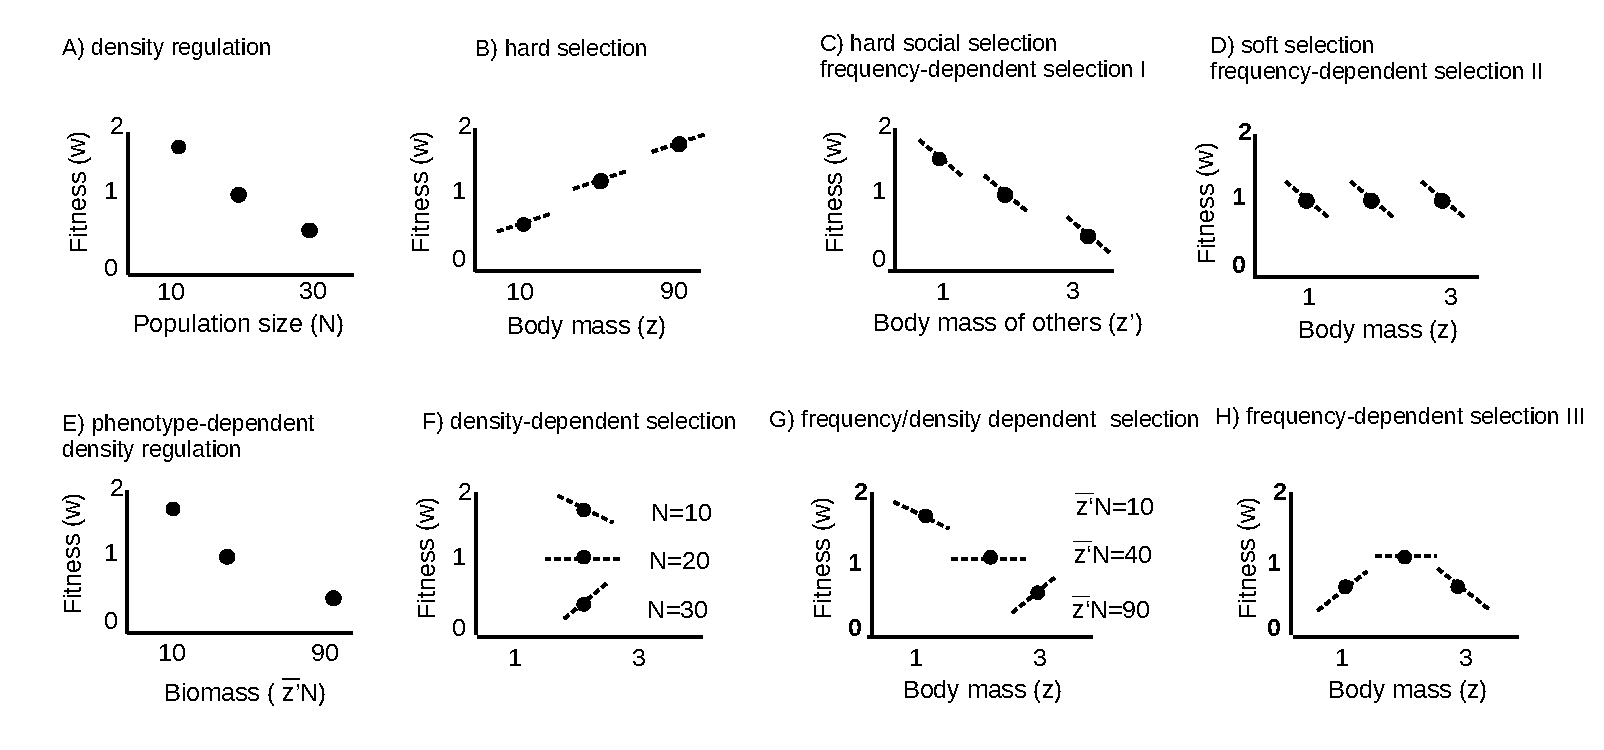
\includegraphics[width=15cm, height=8cm]{Figures/Fig2.pdf}
	\caption{The different social environment effects on the eco-evolutionary dynamics of populations. Here $w$ is used to denote the fitness of individuals, $z$ their phenotypes (e.g. body mass), $N$ the number of individuals in the population, $z'$ the phenotypes of other individuals in the population, and $\bar{z'}$ the average phenotype in the social environment. Black dots represent the average phenotype $\bar{z}$ and fitness $\bar{w}$ for a selection episode, and dashed lines represent the phenotype-fitness relationship within each selection episode. (A) Density regulation, where the number of individuals ($N$) affects the fitness ($w$) of all individuals independent of phenotype. (B) `Hard' selection where the relationship between an individual's phenotype (e.g. body mass) and its own fitness is independent of the social environment (i.e. frequency- and density-independent selection). (C) `Hard' social selection (frequency-dependent selection I), where the phenotype of other individuals (e.g. their body mass) in the population ($z'$) affects individual absolute fitness ($w$), causing the mean phenotype in the social environment to affect population size through its (hard selection) effects on mean fitness. (D) `Soft' social selection, where the fitness of a phenotype is relative to the phenotype of other individuals with whom it interacts (i.e. dashed lines). (E) Phenotype-dependent density regulation, where the impact an individual has on the absolute fitness of others depends upon its phenotype (i.e. body mass), and so in this scenario the effect of population size on fitness ($w$) is moderated by the average phenotype in the population ($\bar{z'}N$, e.g. population biomass). (F) Density-dependent selection, where the within-episode relationship between an individual's phenotype ($z$) and its absolute fitness ($w$) depends upon the number of individuals in the population ($N$) but not on the mean phenotype in the population. (G) Density- and frequency-dependent selection, where the within-episode relationship between an individual's phenotype ($z$) and its absolute fitness ($w$) depends upon both the number of individuals ($N$) and the mean phenotype (e.g. body mass) in the population ($\bar{z}$). (H) Frequency-dependent selection III, where the relationship between an individual's phenotype and its absolute fitness ($w$) depends upon the mean phenotype in the population ($\bar{z}$), but is independent of the number of individuals in the population ($N$).} \label{fig:selection}
\end{figure}

\newpage
\begin{figure} [H]
	\centering
	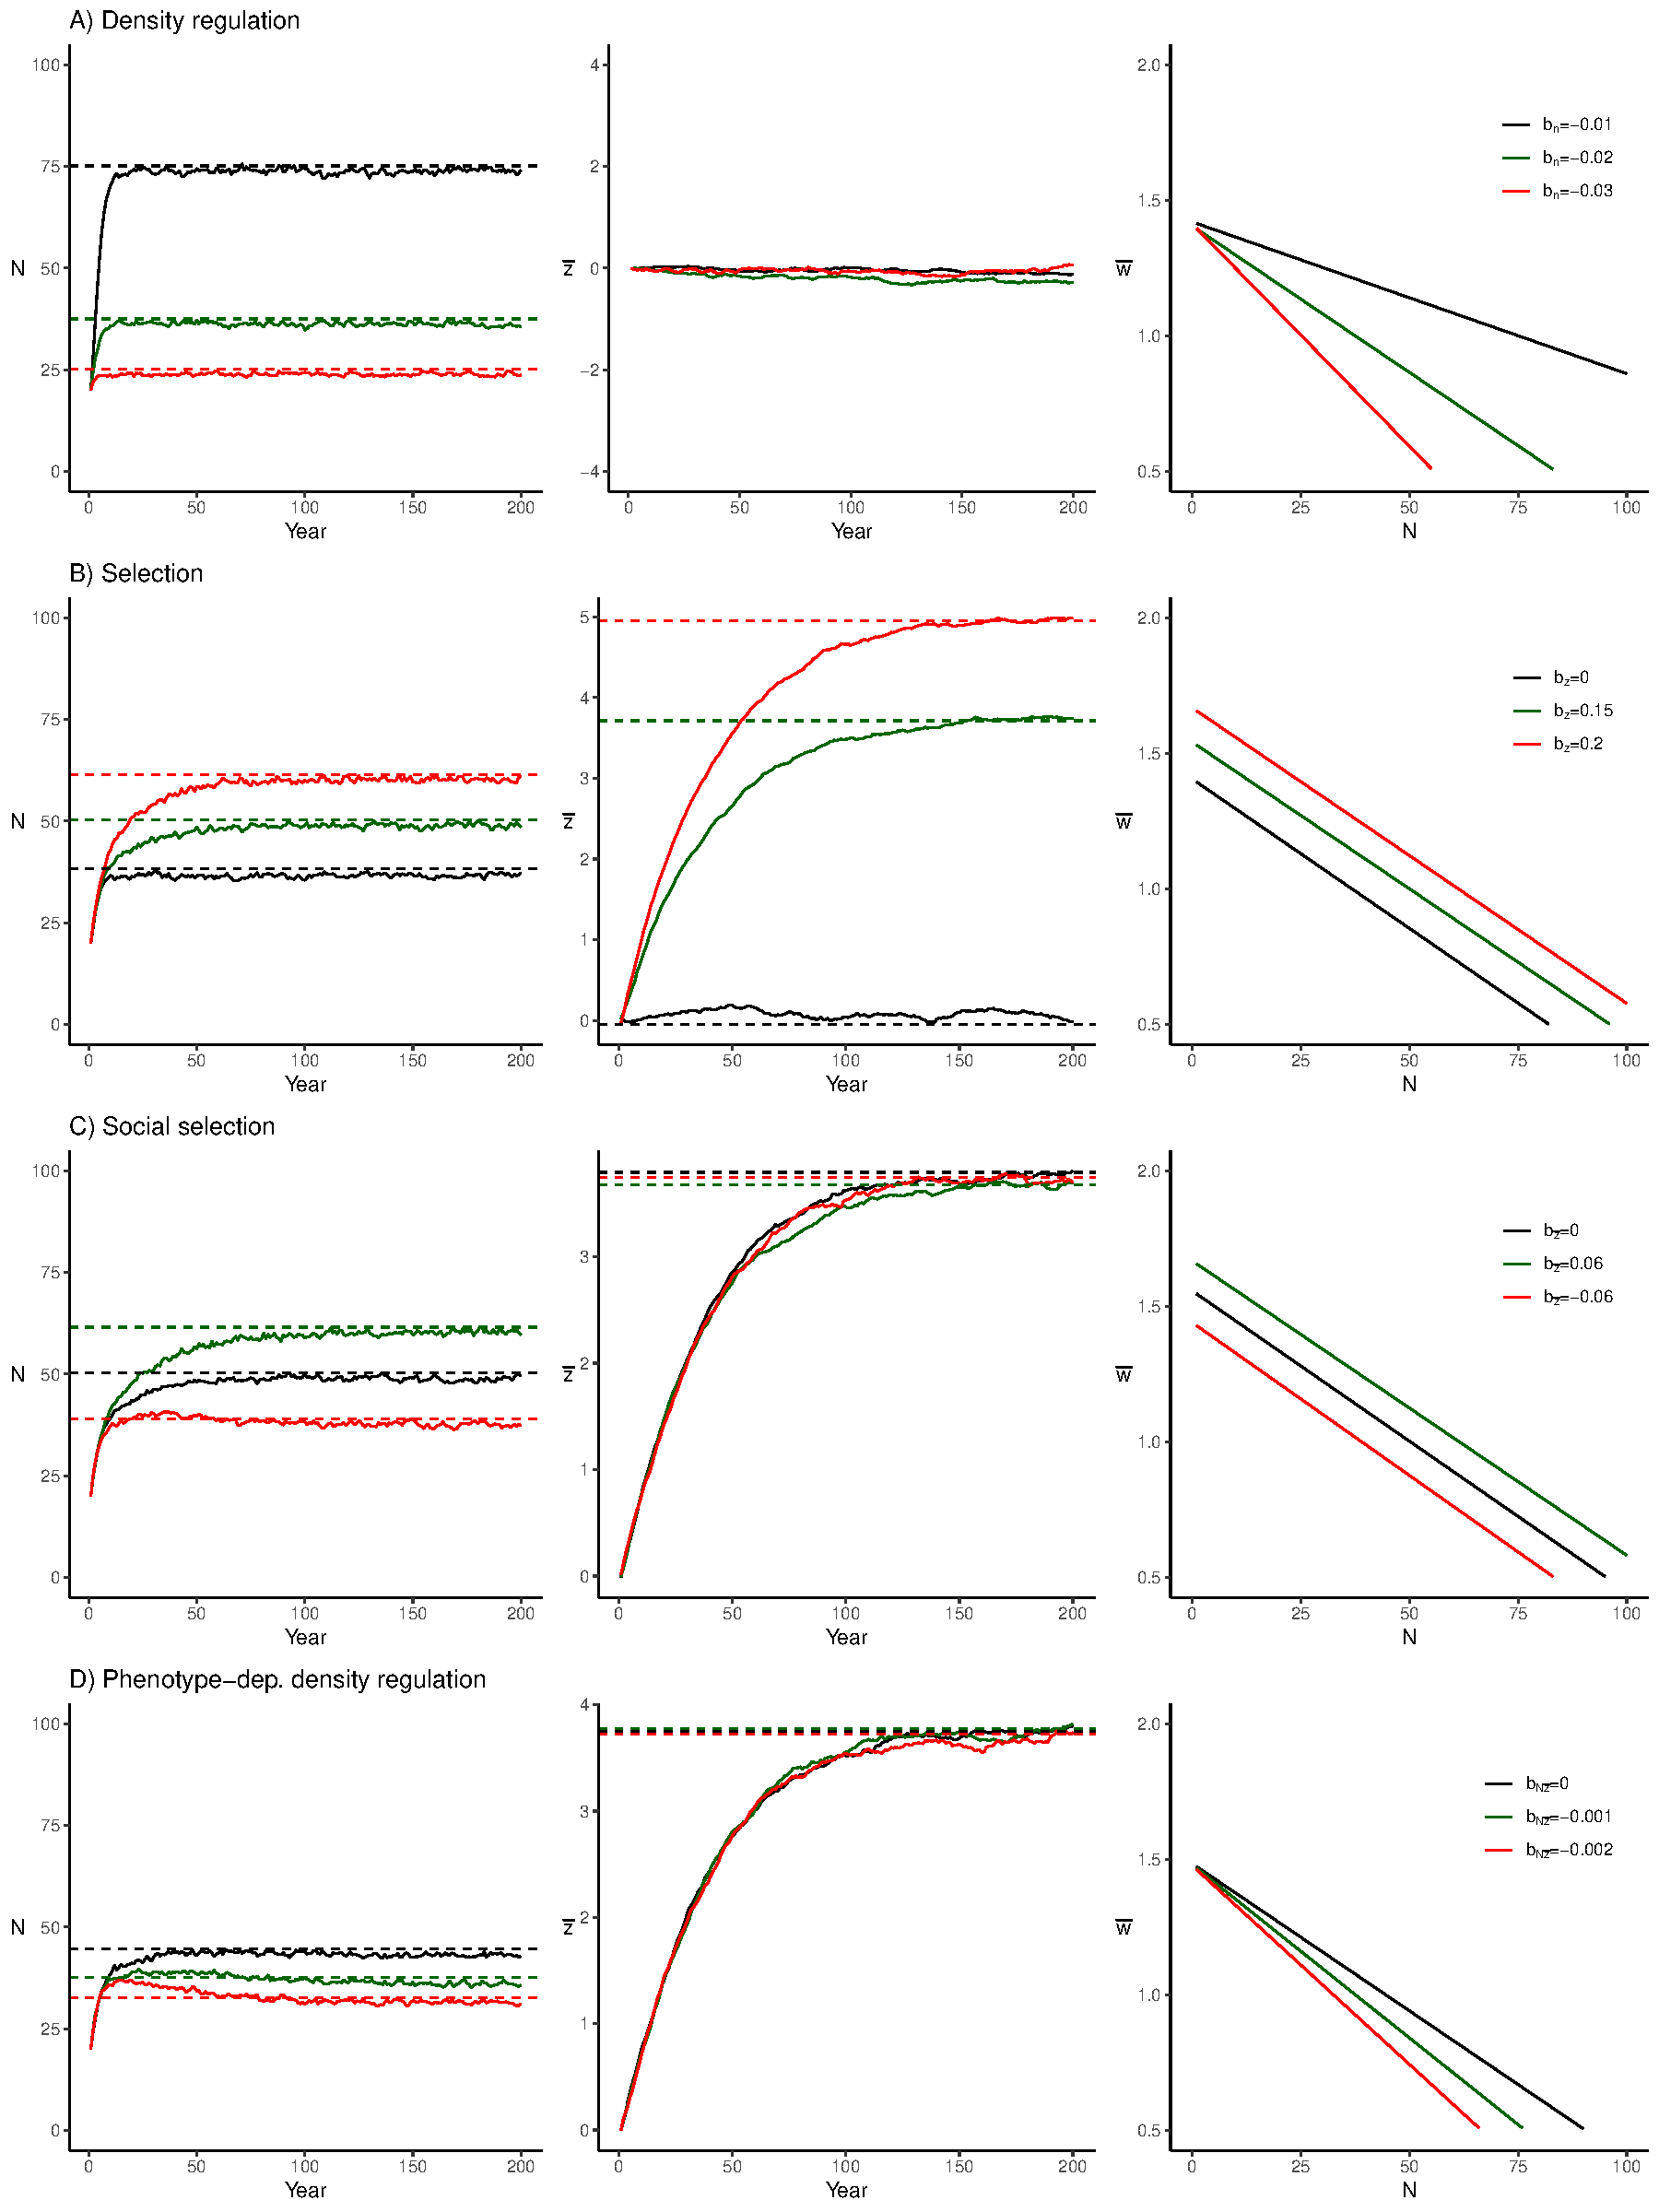
\includegraphics[width=12cm, height=16cm]{Figures/Fig3.pdf}
	\caption{Individual-based simulations results for scenarios 1-4 involving density regulation, direct selection on the phenotype, 'hard' social selection and phenotype-dependent density regulation. The left-hand graphs (labelled (i)) show the trajectory of population size (N) each Year until it arrives at its equilibrium, the middle graphs (labelled (ii)) show the trajectory of the mean phenotype ($\bar{z}$) each Year evolving towards its equilibrium, and the right hand graphs (labelled (iii)) show a population's growth rate ($\lambda$) as a function of population size (N). In each scenario we varied a specific parameter while keeping the others constant (see Table 2 for details of all simulation parameters). The values for the parameters that were changed in each case are presented in the legends in the right-hand graphs. Hence the lines of different colours represent different parameter values for each scenario, and horizontal dashed lines of each colour are the equilibrium population sizes and mean phenotypes predicted from the statistical model estimates. (A) Scenario 1, density regulation and no selection on the phenotype (i.e. where the average phenotype of the population matches the optimum phenotype and there is no phenotypic evolution - see A(ii)). The strength of density regulation (colour-coded changes in $b_n$ depicted in A(iii)) results in different equilibrium population sizes (A(i)). (B) Scenario 2, 
`hard' direct selection on the phenotype (e.g. the introduction of a new resource resulting in selection for the ability to exploit it), where the different coloured lines represent different strengths of directional selection ($\beta_{{z}}$) on the phenotype. Evolution gradually shifts the mean phenotypic values closer to the equilibrium phenotype (B(ii)), resulting in different equilibrium population sizes (B(i)), despite the slope of the effect of population size on mean fitness being the same throughout (B(iii)). (C) Scenario 3, 
`hard' social selection or frequency-dependent selection I, where the mean phenotype of individuals in the social environment affects individual absolute fitness, with different strengths of selection ($\beta_{\bar{z}}$). This affects the equilibrium size of the population (C(i)) because it influences the mean fitness of the population (different elevations in C(iii)), even though the equilibrium phenotype remains the same (C(ii)). (D) Scenario 4, phenotype-dependent density regulation, where the effect of population size on average individual fitness depends upon the mean phenotype in the population, with different degrees of density regulation ($\beta_{{N\bar{z}}}$). Populations with the same mean phenotype (D(ii)) can have different equilibrium population sizes (D(i)) when the relationship between population size and mean fitness depends on how the mean phenotype modulates the strength of density regulation (i.e. the slopes in D(iii)).}
	\label{fig:sim2}
\end{figure}

\newpage
\begin{figure} [H]
	\centering
	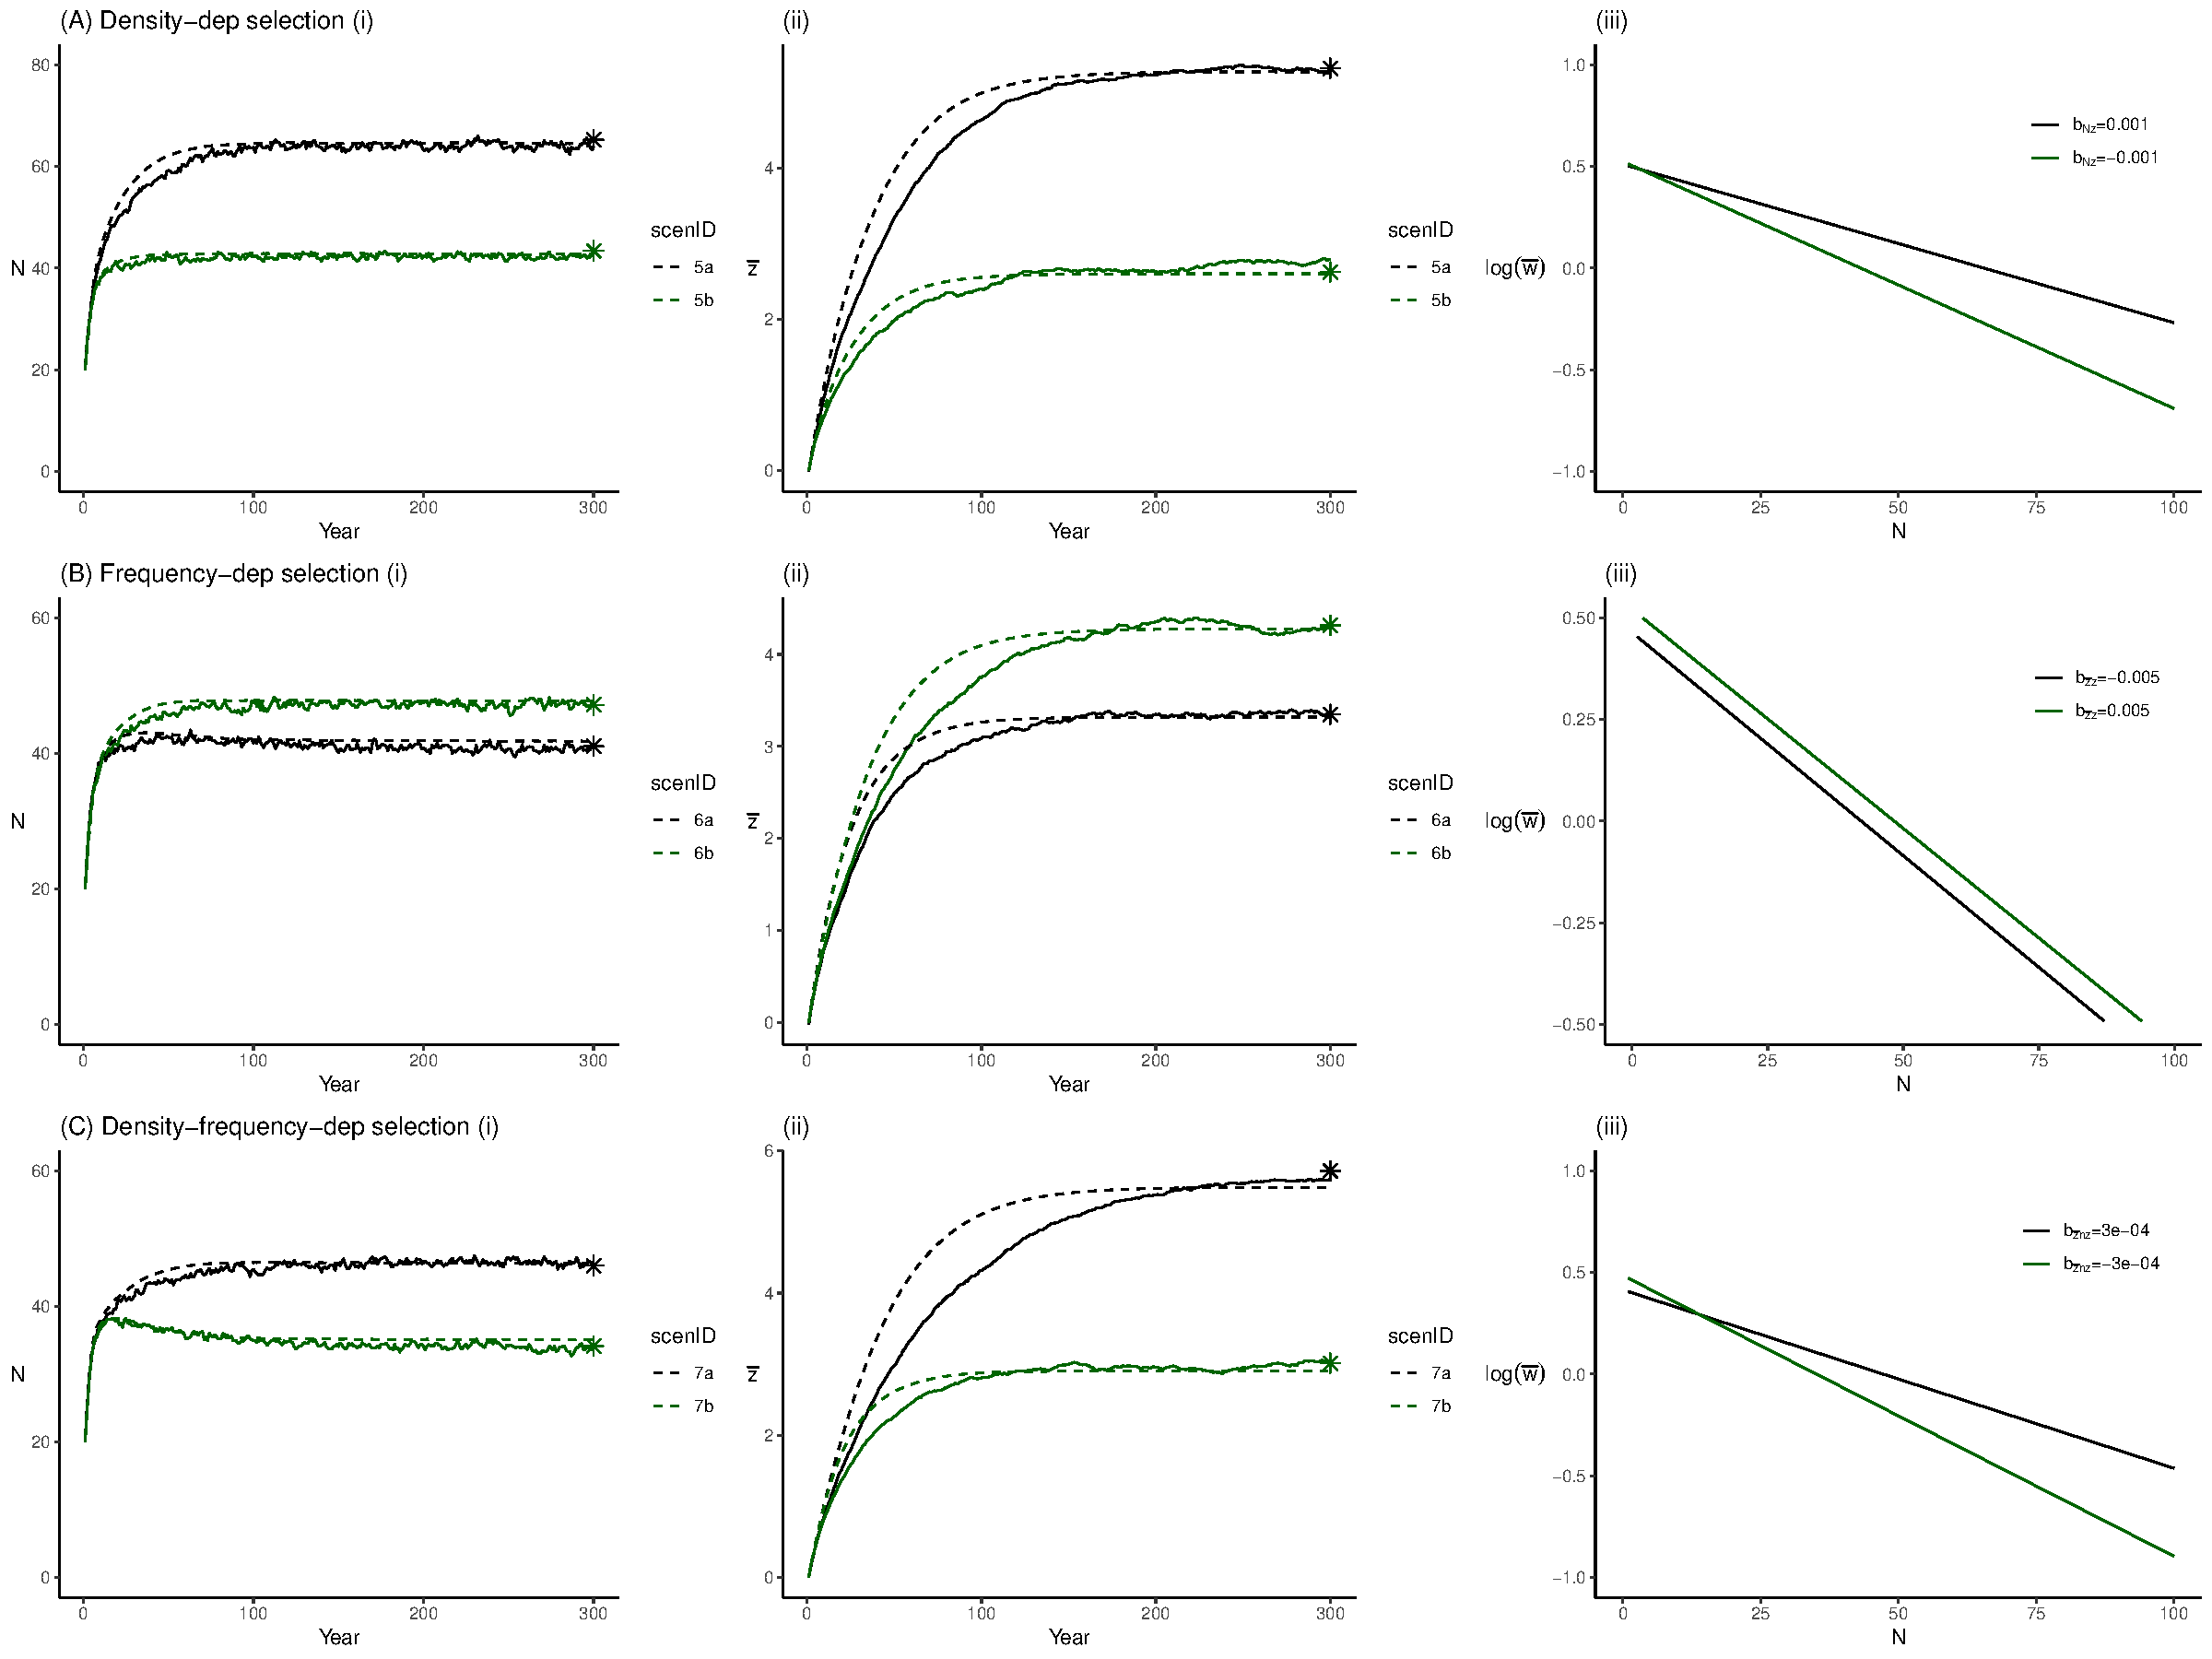
\includegraphics[width=12cm, height=12cm]{Figures/Fig4.pdf}
	\caption{Individual-based simulation results for scenarios 5-7 showing the eco-evolutionary consequences of density-dependent selection (A), frequency-dependent selection II (B), and their interaction (C). As in Figure 3, the left-hand graphs (labelled (i)) show the trajectory of population size over time, the middle graphs (labelled (ii) show the trajectory of the mean phenotype, and the right-hand graphs (labelled (iii)) show the relationship between population density and $\lambda$. In each scenario we varied a specific parameter while keeping the others constant (see Table B3.1 for details of all simulation parameters). Coloured lines represent different parameter values for each scenario, and horizontal dashed lines are the equilibrium population size and mean phenotype predicted from these using the statistical estimates. (A) Scenario 5, density-dependent selection, varies the selection coefficient $\beta_{zn}$ to show how this alters the strength of density regulation (the slopes in A(iii)), with direct consequences for the equilibrium population size (A(i)) and the mean phenotype (A(ii)).(B) Scenario 6, frequency-dependent selection III, varies the coefficient $\beta_{\bar{z}z}$ to demonstrate the consequences for the equilibrium phenotype (B(ii)), as well as for the population size (B(i)) via the effect of the mean phenotype on mean fitness (with no affect on the strength of density regulation - B(iii)). (C) Scenario 7, where these two processes (in A and B) interact resulting in frequency- and density-dependent selection, and varying the strength of the coefficient ($\beta_{\bar{z}nz}$) will determine the interdependence between the mean phenotype (C(ii)) and the equilibrium size of the population (C(i)). The strength of ($\beta_{\bar{z}nz}$) will affect both the mean fitness of a population when its size is very small (the intercepts in C(iii)) and how population size affects the mean fitness of the population (the slopes in C(iii)), which can result in a variety of different effects on the equilibrium population size and mean phenotype (see Figure 4).} 
	\label{fig:sim3}
\end{figure}
\newpage
\begin{figure}  [H]
	\centering
	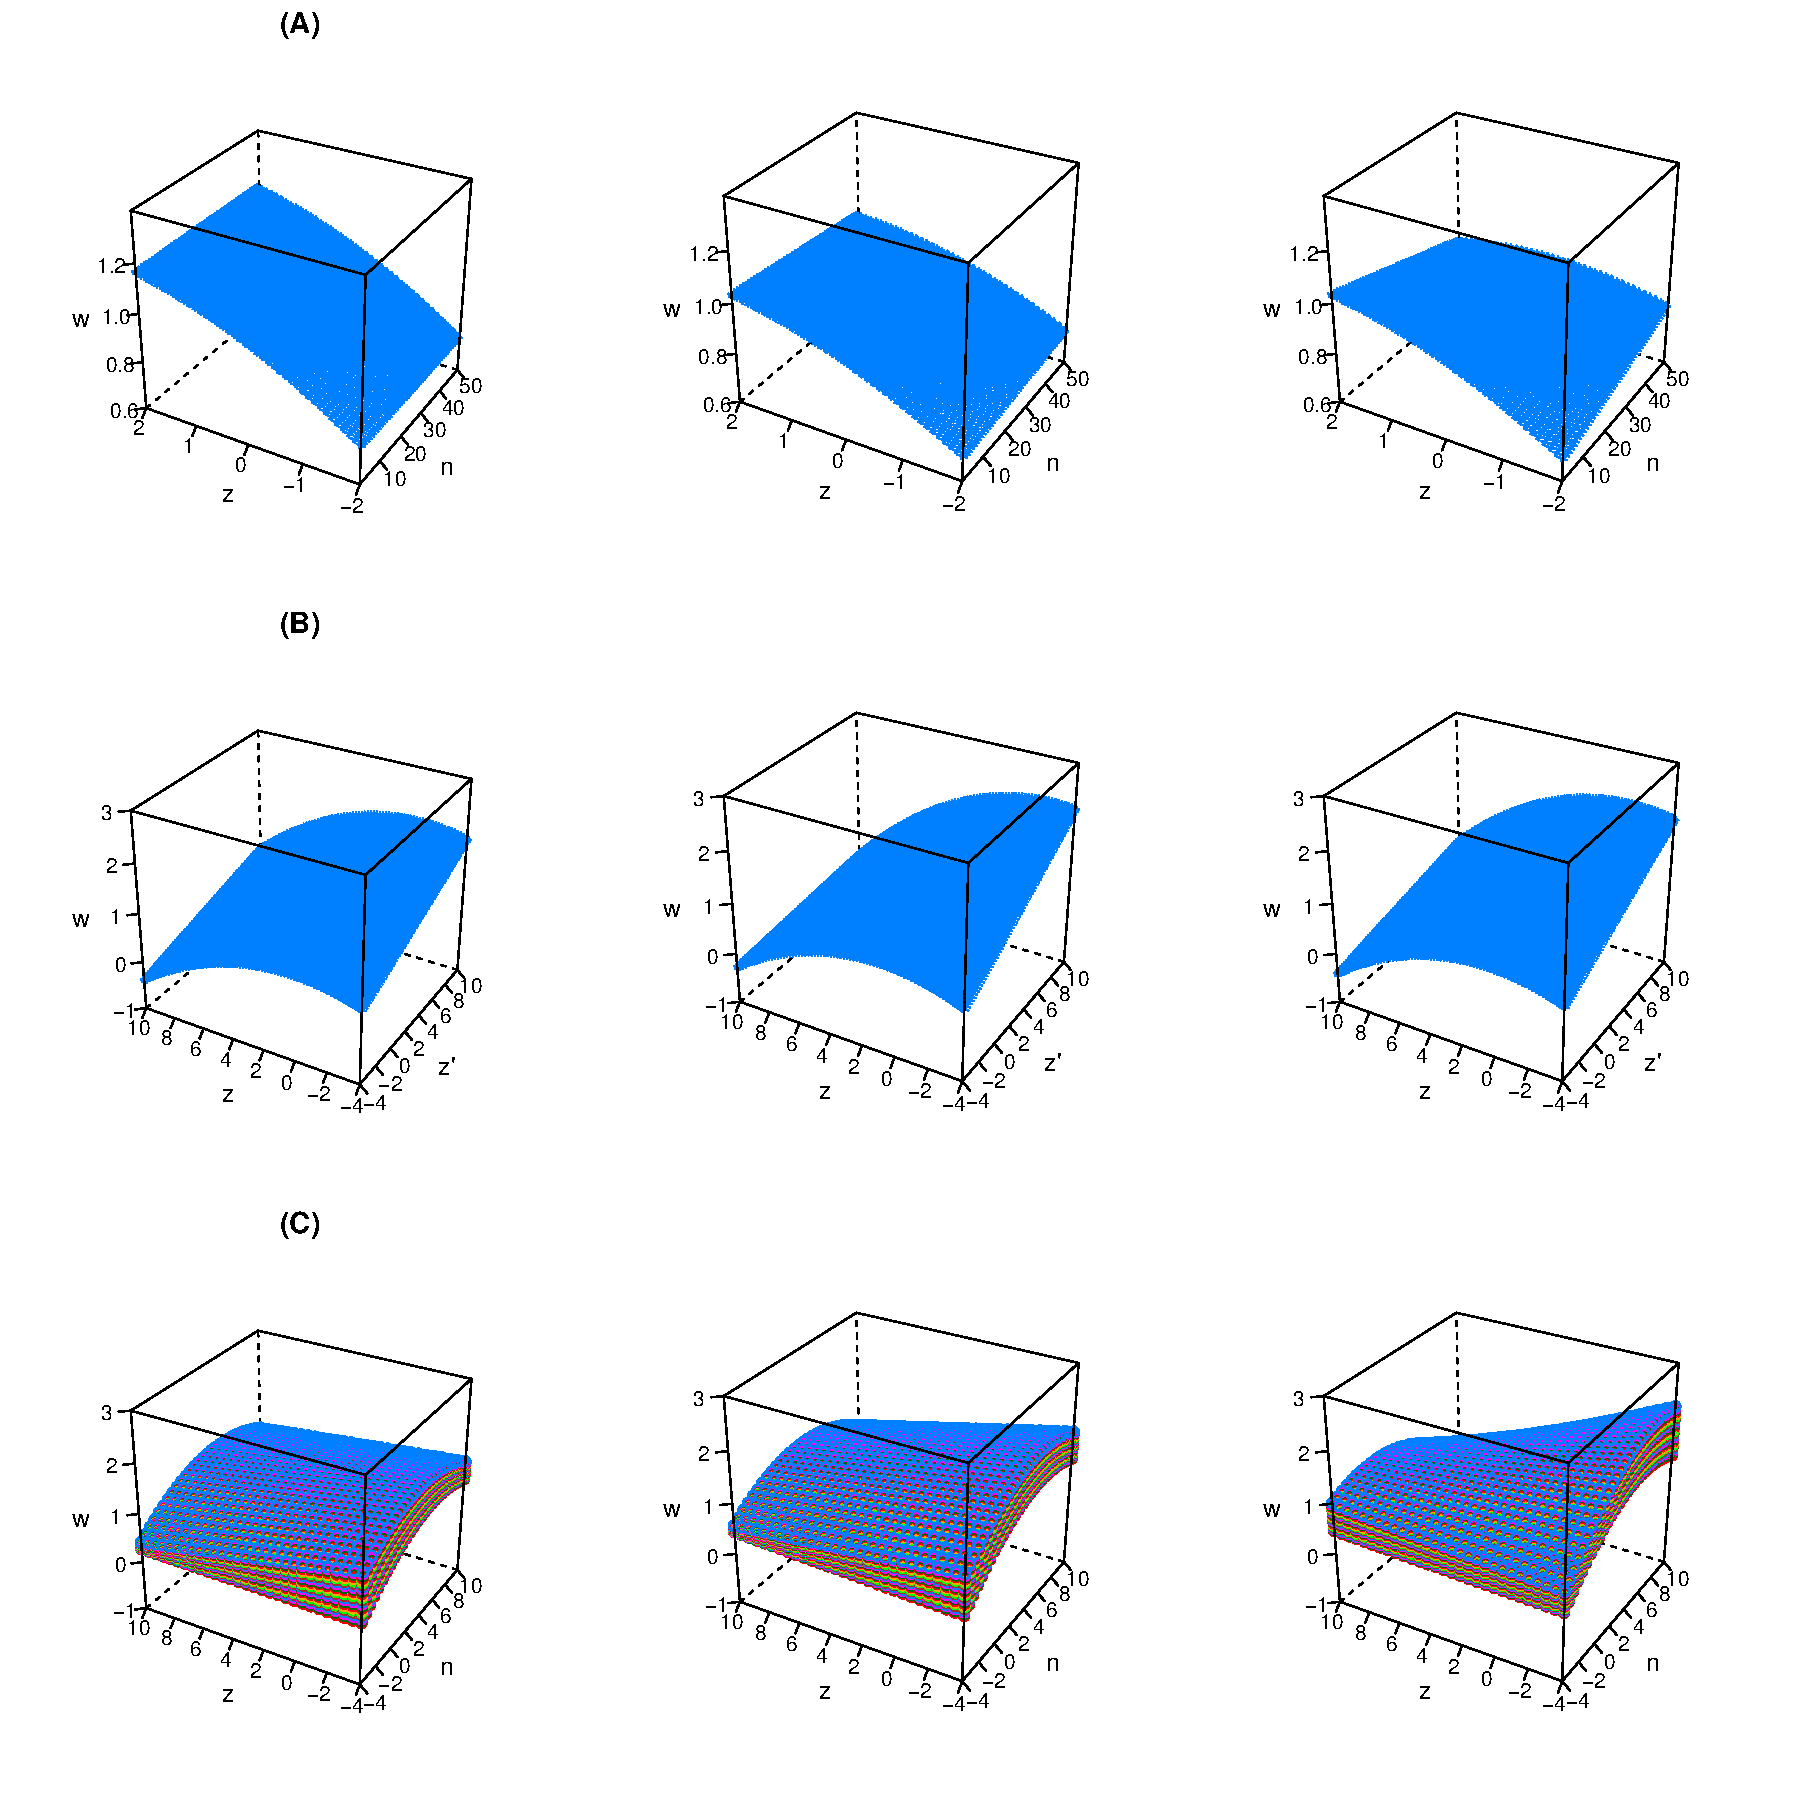
\includegraphics[width=12cm, height=12cm]{Figures/Fig5.pdf}
	\caption{Fitness surfaces for: (A) scenario 5, density-dependent selection; (B) scenario 6 frequency-dependent selection III; and (C and D) scenario 7, frequency- and density-dependent selection. Surfaces show relative fitness (w) to emphasize the effects on selection within each episode. The fitness surfaces correspond to the predictions based upon the multiple regression estimates. Each point on the surfaces represents a different set of simulations with different parameter values for each scenario (see Table B3.1; Figure 3). In (C) the different colours represent a different mean phenotype. In this scenario 7, the fitness surface describing the relationship between an individual's phenotype, its fitness and the average phenotype in the social environment changes depending upon the size of the population.} 
	\label{fig:surface}
\end{figure}


\newpage

\section{Boxes}

\subsection{Box 1: How social interactions mediate eco-evolutionary feedbacks}
\setcounter{figure}{0} 

\noindent Figure B.1 depicts the role of social interactions in mediating eco-evolutionary feedbacks through density- and frequency-dependent processes \citep{Engen2020}. Path 1 (p1) shows how the strength of competition for limited resources determines population size through density regulation \citep{Gilpin1973a}. Change in population size in turn affects density-dependent competition (p2), creating the classic ecological feedback (p1,2) determining the equilibrium size of a population \citep{Travis2013}. If selection is density-dependent (p1,2,3), the size of a population will also have cascading effects on phenotypic selection  \citep{Mueller1997, Boyce1984}. For instance, when populations are large and closer to carrying capacity, investing in somatic growth and competitive behaviours to monopolize resources may be favored. In contrast, when populations are small and resources are abundant, selection may favor smaller individuals that invest in rapid reproduction instead of body size and longer-term competitive ability \citep{Joshi2001, Wright2018, Engen2017}. Density-dependent selection may thus result in the optimal phenotype being dependent upon population size \citep{Anderson1971, Charlesworth1971}. Evolutionary adjustments in the population mean phenotype can, in turn, influence the strength of competitive interactions via the relative frequencies of different phenotypes in the population \citep{Wright1969} (p4,1). Following the example of body size, as competition increases the average individual becomes larger and needs more resources, thus reducing the maximum possible size or carrying capacity of the population \citep{Engen2020}. However, evolution may instead favor social strategies that maximize efficiency of resource use in order to ameliorate the negative fitness effects of competition, potentially increasing the carrying capacity of such populations \citep{macarthur1967theory,  Boyce1984}. When the fitness payoffs of a competitive strategy depends on the strategy of other individuals in the population, the average phenotype in the population can also influence the optimal phenotype for a given individual. This will cause frequency-dependent selection (see Box 2), further affecting both phenotypic evolution (p4,3) \citep{Heino1998} and population size (p4,3,1) \citep{Svensson2018}. Social interactions thus mediate the feedback between ecological and evolutionary dynamics, linking the evolutionary stable phenotype with the equilibrium size of a population (p5).


\begin{figure}[H]
	\renewcommand{\figurename}{Figure B1.}
	\centering
	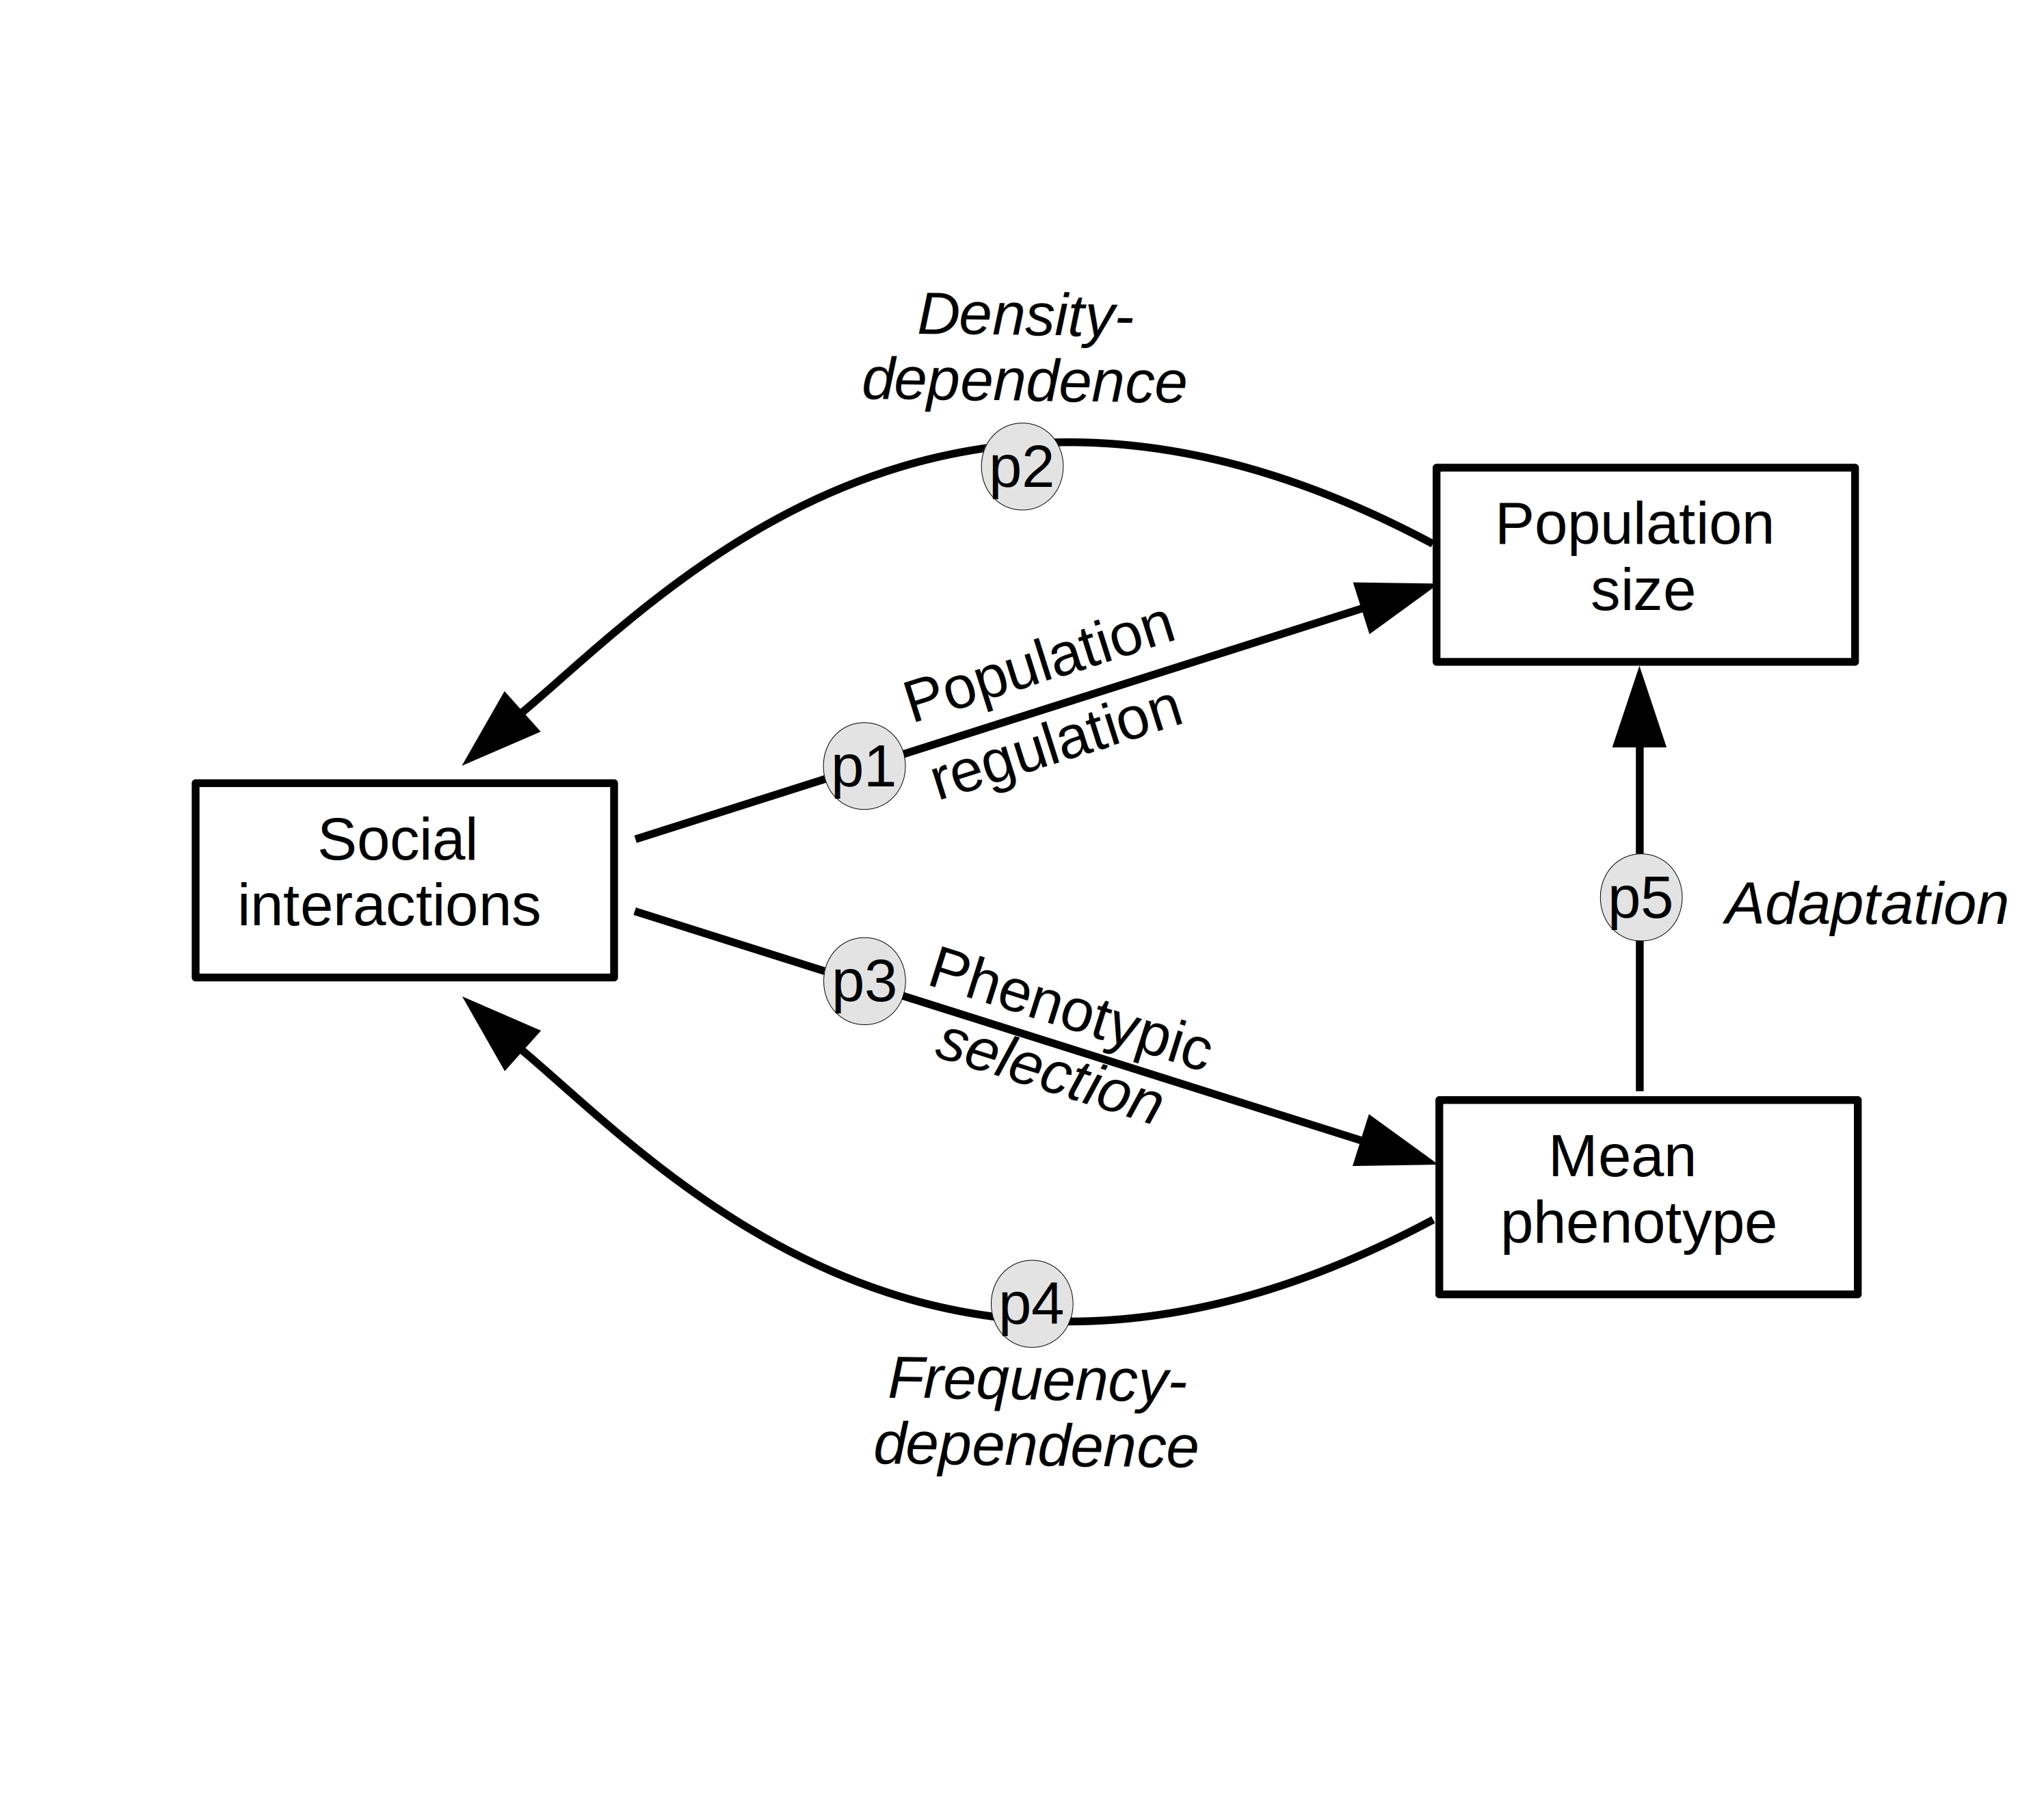
\includegraphics[width=8cm, height=7cm]{Figures/Fig1.jpg}
	\let\nobreakspace\relax
	\caption{Social interactions mediate eco-evolutionary feedbacks}
\end{figure}


\newpage
\subsection{Box 2: The many types of frequency-dependent selection} 
\setcounter{figure}{0}    
\noindent Theoretical models developed in population genetics \citep{Fisher1930, Wright1969}, game theory \citep{MaynardSmith1982, McGill2007, McNamaraLeimar2020} and quantitative genetics \citep{Lande1976, Lande2007, Engen2020} have demonstrated how frequency-dependent selection can affect phenotypic evolution. Classic examples include Fisher's runaway model of sexual selection and the evolution of stable sex ratios \citep{Fisher1930}. Frequency-dependent selection is used to describe many different processes and its definition has been extensively discussed, especially in the context of population genetics and the maintenance of polymorphisms \citep{Ayala1974, Gromko1977, Heino1998}. All the uses of the term “frequency-dependent selection" have in common that the fitness of a phenotype varies with its frequency in the population. However, it is important to make the distinction between the different types of frequency-dependent selection here, because they can have quite different consequences for phenotypic evolution and population dynamics. Here, we make these distinctions from a statistical perspective, based upon whether the effects of the individual's phenotype and its social environment on its fitness are additive (frequency-dependent selection I), relative (frequency-dependent selection II) or interactive (frequency-dependent selection III).

Frequency-dependent selection I (Figure B1 (i) \& (ii)) refers to scenarios in which the effect of the average phenotype in the social environment and the effect of individual's phenotype on its own fitness have additive effects ($\beta_z \mathbf{z} + \beta_{\bar{z}} \mathbf{\bar{z}}$ ). This situation has been shown to result in maladaptation \citep{Lande1976} and can thus affect population dynamics \citep{Lande2007}. In Figure 1C (main text), we describe such frequency dependence I as 
`hard' social selection, because the direct effect of an individual's phenotype on its fitness does not change as a function of the average phenotype in the social environment, but the average phenotype affects the absolute fitness of all individuals. 

Frequency-dependent selection II (Figure B1 (iii) \& (iv)) describes scenarios in which the effect of a phenotype on fitness is relative to the average phenotype in the social environment ($\beta_z [z-\bar{z}]$). This type of frequency-dependent selection includes `soft' selection \citep{Wallace1975, Bell2021}. This can be thought of as a zero-sum game, where a fitness gain of one individual or phenotype results directly in a fitness loss in another, and thus soft selection has no net effect on the mean fitness in the population. Frequency-dependent selection II can also be related to more narrow definitions that require negative frequency-dependent selection to result in the stable coexistence of polymorphisms (i.e. where the fitness of a phenotype decreases with its relative frequency in the population). This process was at the center of early developments of the concept of frequency-dependent selection in game theory and population genetics \citep{MaynardSmith1982, McGill2007, Gromko1977, Ayala1974, Heino1998}. In a quantitative genetic framework, it can formulated as a type disruptive selection \citep{Burger2004}, were the effects of a phenotype depends on the absolute deviation from the average phenotype in the population ($z-\bar{z}^2$). 

Frequency-dependent selection III (Figure B1 (v) \& (vi), and Figure 2G main text) consists of scenarios in which an individual's phenotype interacts with the average phenotype of its social environment to affect its fitness ($\beta_{z\bar{z}} \mathbf{\bar{z}z}$). This results in a warped fitness surface were the direct effect of a phenotype on fitness changes with the average phenotype in the social environment \citep{Araya-Ajoy2020}. This may represent a type of balancing selection \citep{Gromko1977}. For instance, in a scenario where the mean population phenotype becomes larger then individuals with a smaller phenotype will have an advantage, but as the mean phenotype becomes smaller individuals with a larger phenotype will have an advantage (see Figure B1 (vi)).

\begin{figure}[H] 
	\renewcommand{\figurename}{Figure B2.}
	\centering
	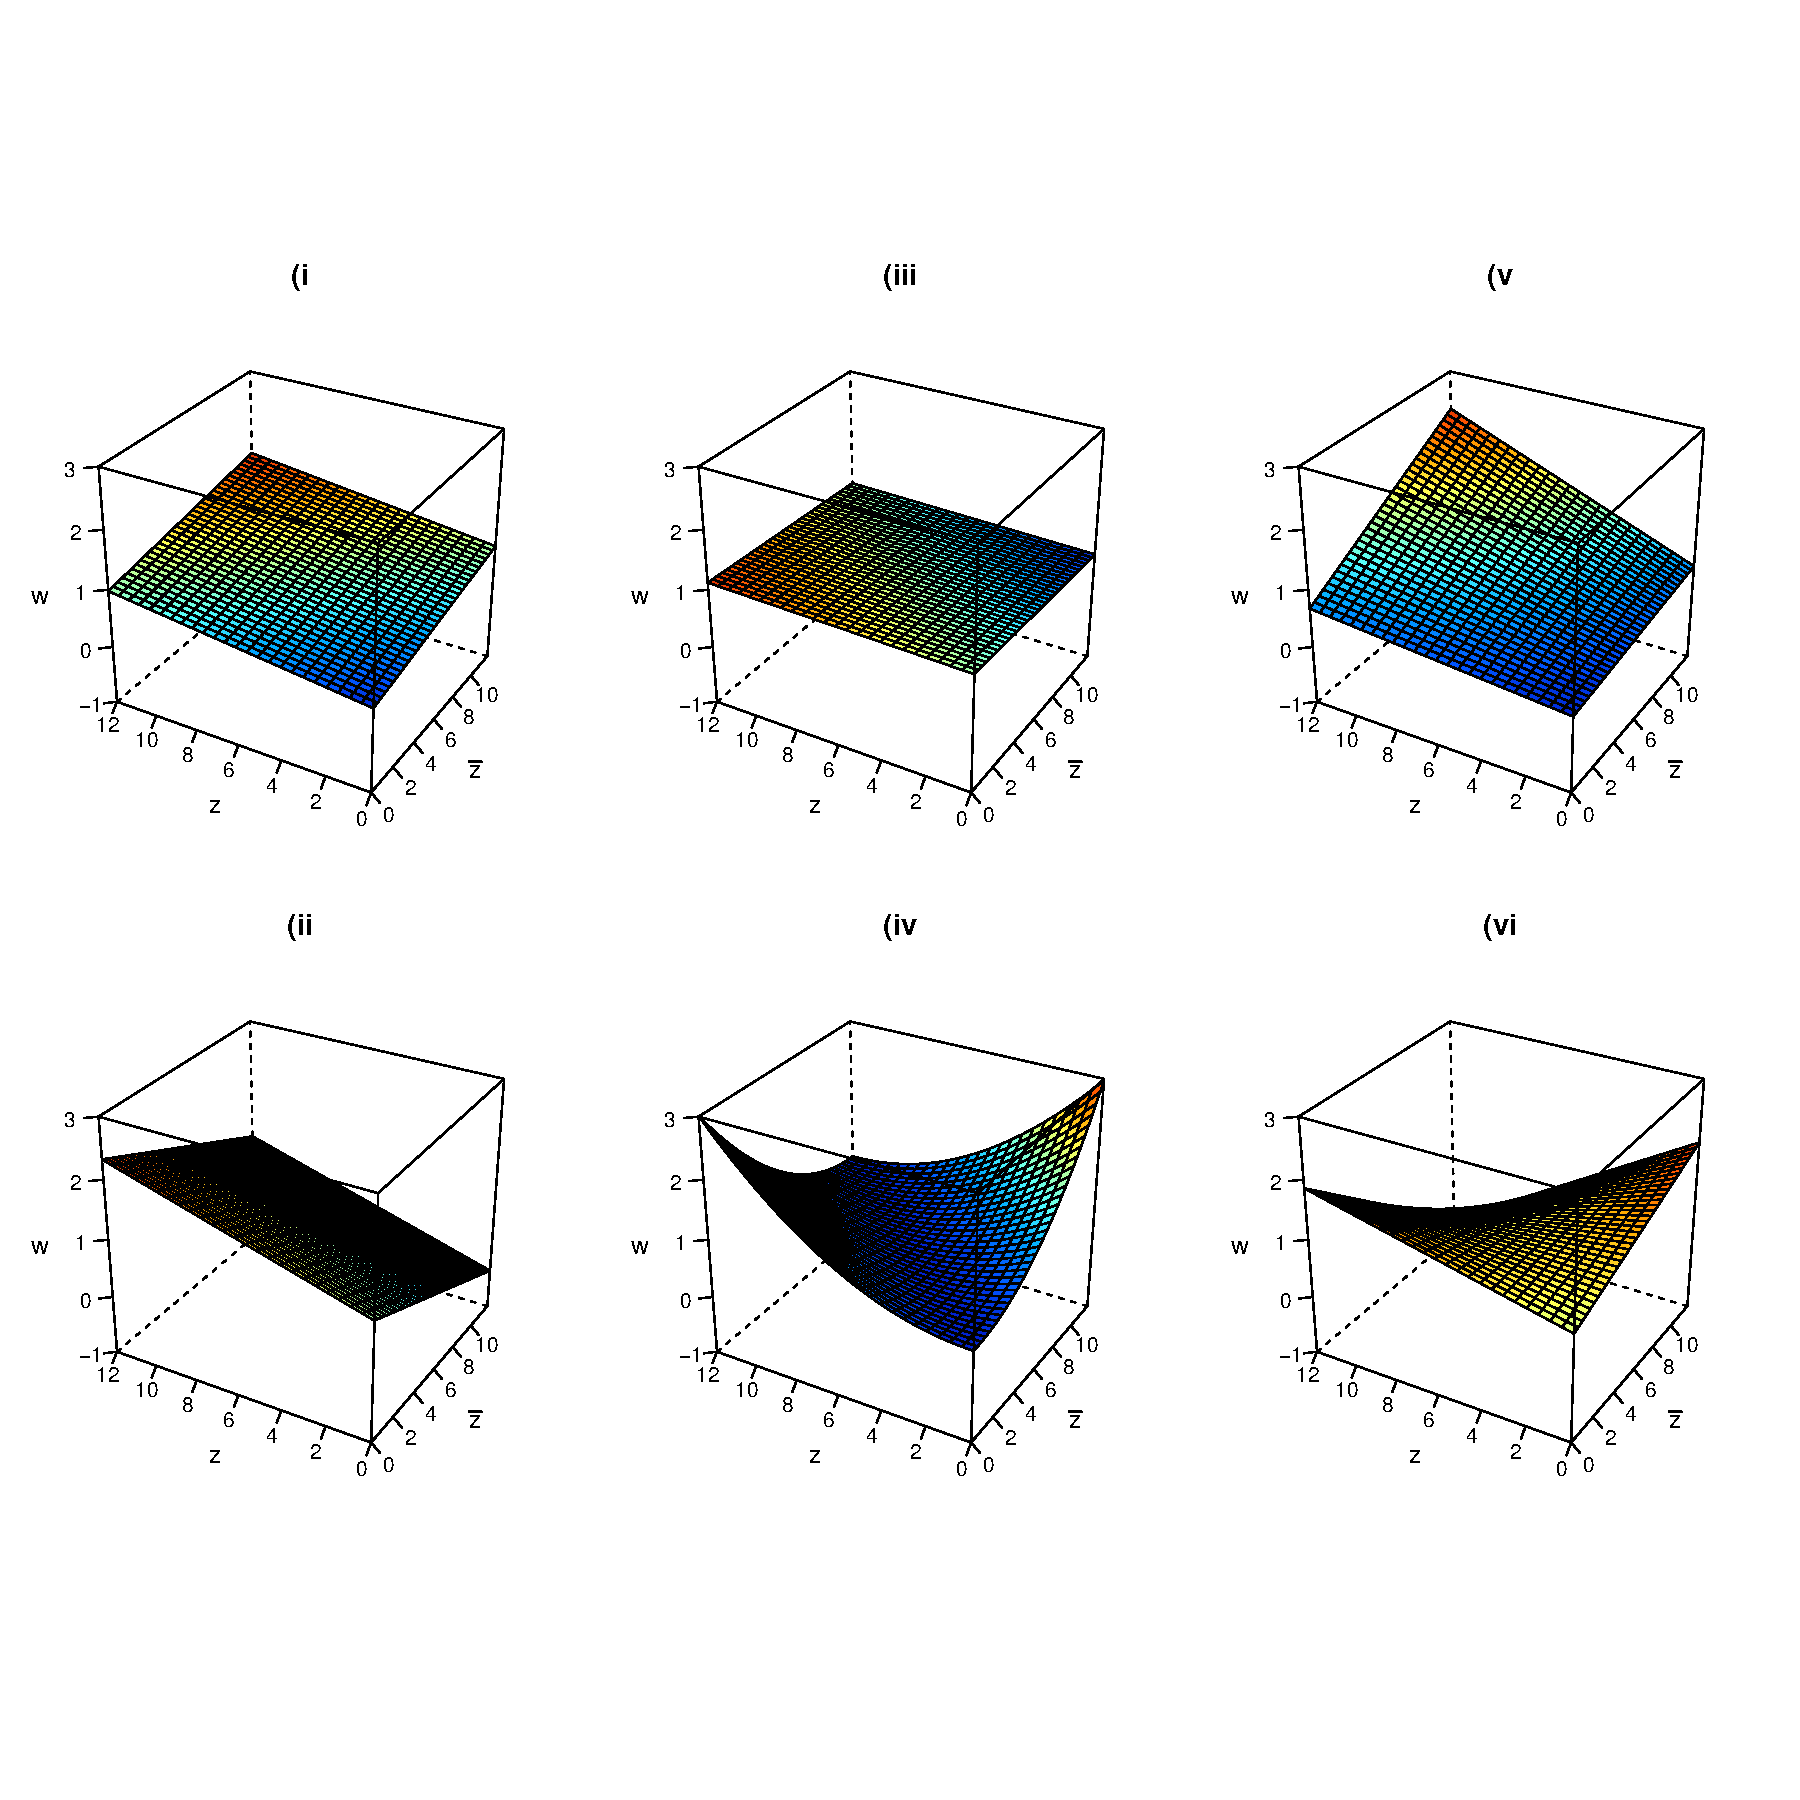
\includegraphics[width=14cm, height=14cm]{Figures/Box2.pdf}
	\let\nobreakspace\relax
	\caption{Fitness surfaces for different types of frequency-dependent selection. The left-hand panels represent scenarios of (i) positive and (ii) negative frequency dependence I, in which the effects of an individual's phenotype and that of its social environment have additive effects on its fitness. The middle panels (iii) and (iv) represent scenarios of frequency-dependent selection II, in which the effects of an individual's phenotype on its fitness are relative to the average phenotype in its social environment, with (iii) a scenario of positive selection for having a higher phenotypic value than that of the average individual in the social environment ($z-\bar{z}$), and (iv) a scenario of negative frequency-dependent selection (and the evolution of polymorphisms) in which the effects of the phenotype depend upon its absolute deviation from the mean phenotype in the social environment ($(z-\bar{z})^2$). The right-hand panels represent scenarios of (v) positive and (vi) negative frequency dependence III, in which an individual's phenotype interacts with that of its social environment to affect its fitness ($\beta_{z\bar{z}} \mathbf{\bar{z}z}$), such that the fitness function depends upon the mean phenotype in the social environment. See Box 2 text for more detail.}
	
\end{figure}


\subsection{Box 3: An eco-evolutionary individual-based simulation}
\setcounter{table}{0}     

\section{Supplementary Appendix I}
 Initial formal models of density-dependent selection \citep{Anderson1971, Charlesworth1971} were based upon the logistic function of population growth. These models were then extended to describe more general patterns of density-dependent population growth rates \citep{Gilpin1973a} and its consequences for phenotypic evolution \citep{Gilpin1976}. Extensions of the logistic model allowed different growth trajectories for populations with the same carrying capacity (\textit{K}) by introducing an extra parameter, $\theta$ \citep{Lande2003}. If $\theta$ equals 1 then the model is simply the logistic density dependence model, but larger values of $\theta$ indicate stronger density regulation closer to \textit{K}, whereas for lower values of $\theta$ then the maximum population growth rate occurs when N is less than \textit{K}/2. The dynamics of population growth in our individual-based simulations are best approximated by a $\theta$ logistic model with $\theta$ values above 1 (Figure \ref{fig:growth}). These types of population dynamics are characteristic of vertebrates, where populations grow quickly towards their equilibrium size and then population growth ceases rather abruptly, because resource monopolization (e.g. territoriality) tends to mediate competitive interactions in these systems \citep{Gilpin1973a}. 
 
 \begin{figure}[H] 
 	\centering
 	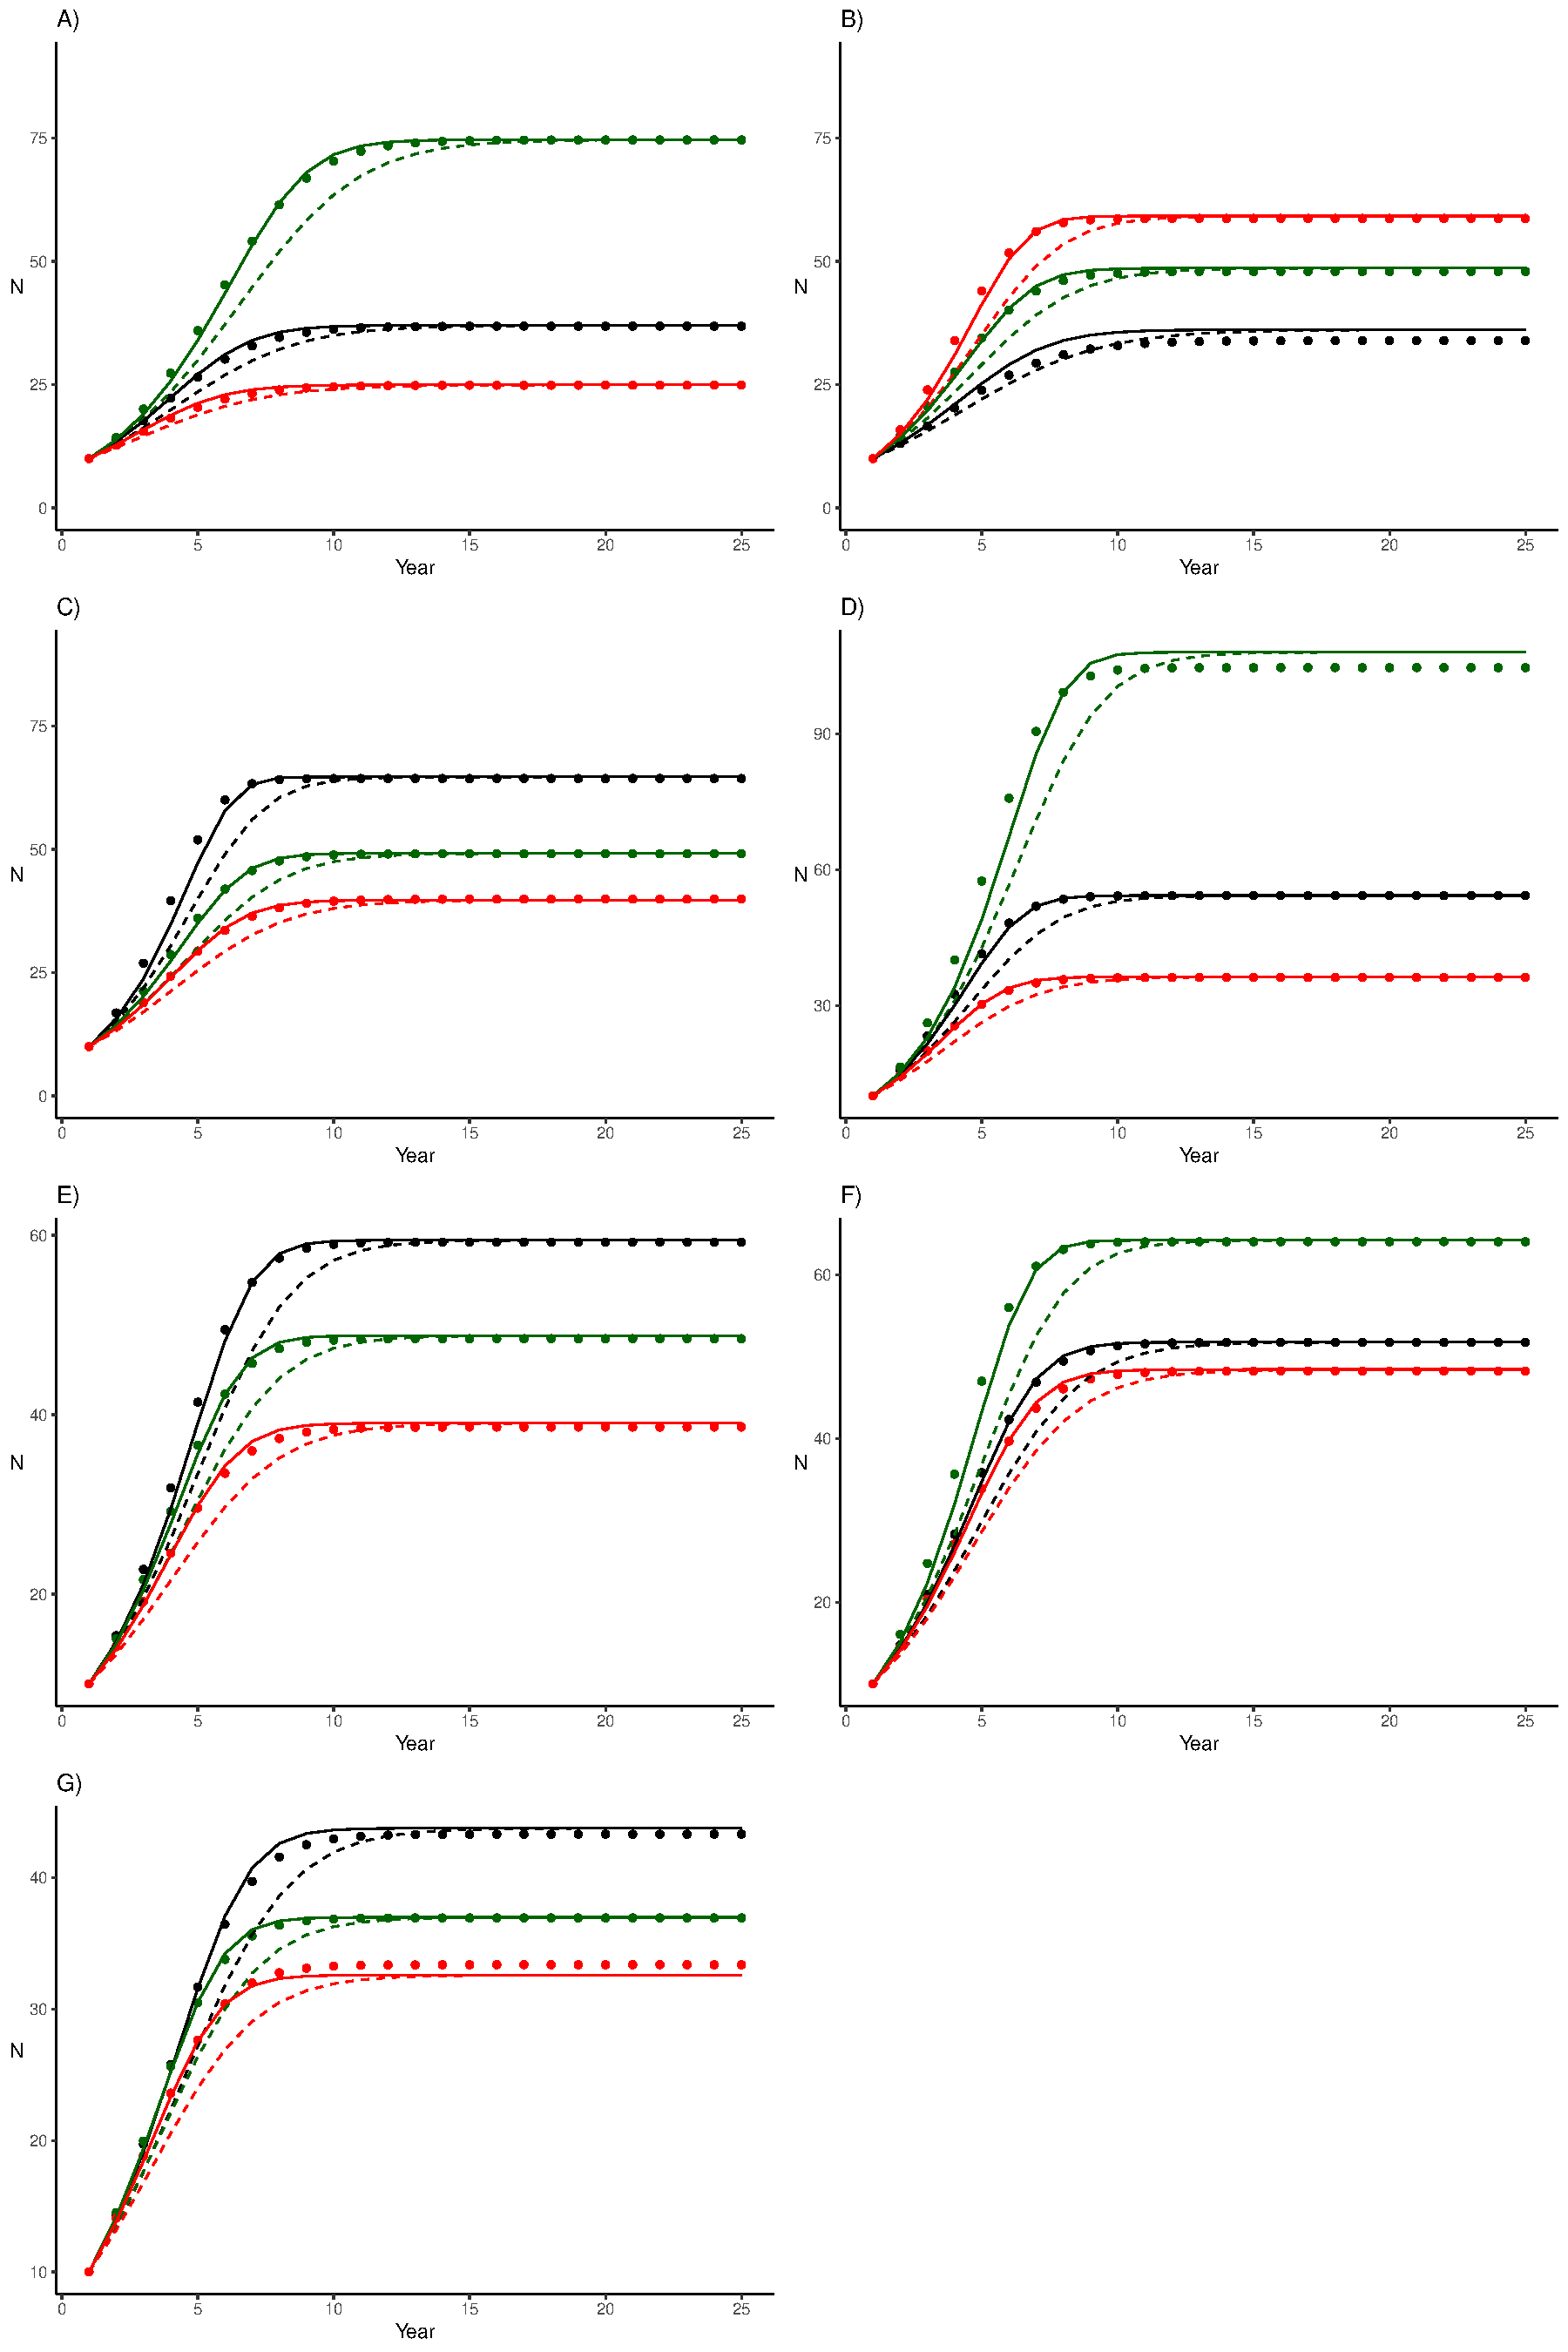
\includegraphics[width=12cm, height=18cm]{Figures/FigS4.pdf}
 	\caption{Predicted changes in population size using the multiple regression estimates (circles), a logistic model (dashed lines) and the theta logistic model of population growth (solid line). Colours represent the different simulations for each scenario (see Table B3.1). (A) Scenario 1 with density regulation; (B) Scenario 2 with selection; (C) Scenario 3 with social selection; (D) Scenario 4 with phenotype dependent regulation; (E) Scenario 5 with density dependent-selection; (F) Scenario 6 with frequency-dependent selection; and (G) Scenario 7 with frequency- and density-dependent selection.} 
 	\label{fig:growth}
 \end{figure}
 
 \section{Supplementary Material}
 \subsection{Appendix 1: Full equation for individual based simulation}
 
 \begin{subequations}
 	\begin{gather}
 	\bm{r}\sim Poisson(e^{R_{0} + b_{n} \bm{n} + b_{z} \bm{z} + b_{q} \bm{z^2} + b_{\bar{z}} \bm{\bar{z}} + b_{n \bar{z}} \bm{n\bar{z}} + b_{z\bar{z}}  \bm{z\bar{z}} + b_{zn}  \bm{zn} + b_{zn \bar{z}} \bm{zn\bar{z}}+  \bm{e}}), \tag{B3.1a}\label{full sim a} \\
 	\bm{s}\sim Bern(\frac{1}{e^{\bar{p}}}). \tag{B3.1b}\label{full sim b}
 	\end{gather}
 \end{subequations}
 
 Where $R_0$ is the average recruit production in the population when it is very small. Population size effects on mean fitness is described by the density regulation coefficient $b_{n}$. The number of recruits an individual produces can be affected by its own phenotype as a function of the linear ($b_z$) and quadratic ($b_q$) effects of the phenotype on fitness. The number of recruits produced by an individual can also depend upon the (average) phenotype ($\bar{z}$) of the individuals in the population modulated by the coefficient $b_{\bar{z}}$. Furthermore, the average phenotype in the population can also modulate the strength of density regulation as a function of the interaction coefficient $b_{n\bar{z}}$. The optimal phenotype can depend upon the number of individuals in the population ($b_{zn}$), and also upon the mean phenotype in the population ($b_{z\bar{z}}$). Ultimately the relation between phenotype and fitness may also depend on an interaction between the number of individuals and the phenotype of the average individual in the population ($b_{zn\bar{z}}$).
 
 
 \subsection{Appendix 2: Supplementary equations for the density-dependent selection scenario}
 
 Equilibrium population size when there is density dependent selection

 \begin{equation}
 \hat{n} = -\frac{2\beta_{n}\beta_{q} - \beta_{zn}\beta_{z} - 2 \sqrt{\beta_{zn}^2\beta_{q}^2 \sigma^2_z + \beta_{n}^2\beta_{q}^2-\beta_{n}\beta_{zn}\beta_{q}\beta_{z} + \beta_{zn}^2\beta_{q}\beta_{0}}}{\beta_{zn}^2} ,
 \end{equation}

 \noindent Equilibrium phenotype when there is density dependent selection
  \begin{equation}
 \hat{z} = -\frac{2\beta_{n}\beta_{q} + \sqrt{\beta_{zn}^2\beta_{q}^2 \sigma^2_z + \beta_{n}^2\beta_{q}^2-\beta_{n}\beta_{zn}\beta_{q}\beta_{z} + \beta_{zn}^2\beta_{q}\beta_{0}}}{\beta_{zn}\beta_{q}} ,
 \end{equation}
 
 
\end{document}

